% UG project example file, February 2024
%
%   Added the "online" option for equal margins, February 2024 [Hiroshi Shimodaira, Iain Murray]
%   A minor change in citation, September 2023 [Hiroshi Shimodaira]
%
% Do not change the first two lines of code, except you may delete "logo," if causing problems.
% Understand any problems and seek approval before assuming it's ok to remove ugcheck.
\documentclass[logo,bsc,singlespacing,parskip,online]{infthesis}
\usepackage{ugcheck}


% Include any packages you need below, but don't include any that change the page
% layout or style of the dissertation. By including the ugcheck package above,
% you should catch most accidental changes of page layout though.

\usepackage{microtype} % recommended, but you can remove if it causes problems

% \usepackage[numbers]{natbib} % for numerical citations
\usepackage[round]{natbib} % recommended for citations

\usepackage{booktabs}
\usepackage{makecell}
\usepackage{multirow}
\usepackage{amssymb}
\usepackage{amsmath}
\usepackage{tikz}
\usetikzlibrary{positioning, shapes.geometric, arrows.meta}

\begin{document}
\begin{preliminary}

\title{Creating an LLM Tutor with User-Editable Representations}

\author{Francesco La Rosa}

% CHOOSE YOUR DEGREE a):
% please leave just one of the following un-commented
%\course{Artificial Intelligence}
\course{Artificial Intelligence and Computer Science}
%\course{Artificial Intelligence and Mathematics}
%\course{Artificial Intelligence and Software Engineering}
%\course{Cognitive Science}
%\course{Computer Science}
%\course{Computer Science and Management Science}
%\course{Computer Science and Mathematics}
%\course{Computer Science and Physics}
%\course{Software Engineering}
%\course{Master of Informatics} % MInf students

% CHOOSE YOUR DEGREE b):
% please leave just one of the following un-commented
%\project{MInf Project (Part 1) Report}  % 4th year MInf students
%\project{MInf Project (Part 2) Report}  % 5th year MInf students
\project{4th Year Project Report}        % all other UG4 students


\date{\today}

\abstract{
Recent advances in Large Language Models (LLMs) have enabled flexible, conversational tutoring systems, yet these systems often operate as "black boxes" with opaque representations of the learner's knowledge and the pedagogical curriculum. This lack of transparency limits the student's ability to understand their own progress or correct the system's misconceptions about them. We present an LLM-based tutoring system that makes both the curriculum structure and the learner model explicit and user-editable. We hypothesise that transparency (letting students see these representations) and control (letting students modify them) improve learning outcomes by enabling error correction, structured adaptation, and increased user agency. We evaluate this hypothesis through a controlled study comparing our approach against a baseline that mirrors current state-of-the-art systems, measuring both learning gains and pedagogical effectiveness.
}

\maketitle

\newenvironment{ethics}
   {\begin{frontenv}{Research Ethics Approval}{\LARGE}}
   {\end{frontenv}\newpage}

\begin{ethics}
This project obtained approval from the Informatics Research Ethics committee.\\
Ethics application number: 413322\\
Date when approval was obtained: 2025-12-08\\
The participants' information sheet and a consent form are included in the appendix.

\standarddeclaration
\end{ethics}


\begin{acknowledgements}
Any acknowledgements go here.
\end{acknowledgements}


\tableofcontents
\end{preliminary}


\chapter{Introduction}

The integration of Large Language Models (LLMs) into educational technology has transformed automated tutoring. Systems like ChatGPT and Khanmigo offer a fluidity of conversation that was previously difficult for computers to achieve \citep{openai2025studymode,khanmigoParents}. They can generate explanations on demand, adapt to student inquiries, and cover a wide range of topics. However, this conversational flexibility comes at a significant cost: opacity. These systems operate as "black boxes," generating pedagogical responses without revealing the internal logic that drives them. The student is left in a position of dependency, receiving instruction without insight into why a particular topic was chosen or what the system believes they have mastered.

This lack of transparency creates a critical barrier to effective learning. In a human tutoring scenario, the model of the student's knowledge is often negotiated. A student can correct a tutor who wrongly assumes they are unfamiliar with a prerequisite. In current LLM-based systems, this model is implicit. It hides within the neural network's activation states or the unstructured text of the conversation history \citep{chen2024chattutor}. If the system misinterprets a student's struggle as a lack of knowledge rather than a simple mistake, the student cannot inspect this assumption or correct the record. The curriculum is similarly invisible. It emerges dynamically turn-by-turn rather than existing as a structured map the learner can consult and audit.

\section{Research Question and Hypothesis}

This thesis investigates whether bridging the gap between the explicit, structured representations of traditional Intelligent Tutoring Systems (ITS) \citep{vanlehn2011relative} and the flexible generation of LLMs can resolve this transparency problem. The internal state of a tutor should be a transparent interface, not a black box. The central research question driving this work is: Does granting users transparency over and control of explicit pedagogical representations improve learning outcomes compared to system-controlled, implicit representations?

The Open Learner Model literature distinguishes two dimensions of user access to system state \citep{bull2007invite, kay2013scrutability}. \textit{Inspectability} (or transparency) refers to whether users can see the system's beliefs about them. \textit{Negotiability} (or control) refers to whether users can challenge or modify those beliefs. Current LLM tutors like ChatTutor \citep{chen2024chattutor} offer partial inspectability for the curriculum (users can view the course plan) but no negotiability (users cannot modify it), and neither inspectability nor negotiability for the learner model (which remains a hidden, narrative summary). This thesis proposes making both representations fully inspectable and negotiable.

We hypothesise that inspectability and negotiability improve learning outcomes through three mechanisms. First, error correction: students can fix the system's misunderstandings of their prior knowledge, preventing wasted time on mastered material \citep{bull2010olm}. This mechanism requires negotiability. Second, structured adaptation: tracking mastery at the topic level enables more precise decisions about when to advance and when to remediate. This mechanism requires inspectability. Third, user agency: visualising progress allows students to audit their learning paths and direct their own study \citep{ryan2000sdt}. This mechanism requires both inspectability and negotiability. Based on these mechanisms, we predict that learners with inspectable and negotiable representations will demonstrate greater learning gains than those with hidden or read-only representations.

\section{Approach and Contributions}

To test this hypothesis, we present the design and evaluation of a new tutoring system. Unlike standard conversational agents, the proposed system maintains two explicit artifacts: a Directed Acyclic Graph (DAG) representing the curriculum and a per-topic learner model that tracks mastery confidence. These artifacts are user-editable. A student who feels the system has underestimated their ability can adjust their mastery score, while a student who wishes to skip a topic or add a prerequisite can modify the curriculum graph directly. The system uses a tool-based architecture where pedagogical actions, such as assessing an answer or updating the plan, are separated from the conversational generation, allowing the LLM to act upon these explicit structures.

\noindent This work makes four contributions:
\begin{itemize}
\item A design framework for user-editable pedagogical representations, defining how curriculum graphs and learner models serve as shared interfaces between human and machine.
\item An evaluation methodology focused on learning outcomes through pre- and post-tests, rather than the satisfaction surveys dominating current literature \citep{chen2024chattutor}.
\item A reference implementation demonstrating integration of explicit state management with LLMs.
\item Experimental results comparing this approach against a baseline tutor.
\end{itemize}

\section{Scope and Limitations}

The scope of this research is defined by specific boundaries designed to isolate the effects of transparency and control. We focus on single-session tutoring in technical domains, such as calculus and algorithms, where knowledge structures are well-defined and prerequisite relationships are clear. This constraint allows for rigorous measurement of learning gains within a controlled timeframe. Consequently, this work does not address long-term knowledge retention over weeks or months, nor does it explore the motivational aspects of gamification beyond any motivation that may arise from visualising one's own progress. Our sample consists of university students, which may limit generalisability to other learner populations such as K-12 or professional contexts. The design also assumes that learners will engage with the editing capabilities; some users may prefer to defer control to the system.

Furthermore, our evaluation emphasises multi-turn interaction. Tutoring is inherently a process of unfolding dialogue and iterative adaptation, a dynamic that single-turn benchmarks fail to capture \citep{srinivasa2025tutorbench}. By focusing on the session as the unit of analysis, we aim to understand how explicit representations influence the trajectory of learning, not just the quality of a solitary response. This approach prioritizes depth of interaction over breadth of domain coverage, ensuring that our findings regarding the value of user-editable representations are grounded in the reality of complex learning tasks.

\section{Thesis Outline}

The remainder of this thesis is organised as follows. Chapter 2 establishes the theoretical background, reviewing the history of Intelligent Tutoring Systems and the recent emergence of LLM-based tutors. Chapter 3 surveys related work, positioning our contribution against existing industry and academic systems. Chapter 4 details the system design and methodology, explaining the architecture of the proposed system and the mechanisms for mastery tracking. Chapter 5 describes the experimental design used to validate our hypothesis. Chapter 6 presents the results of this evaluation, analysing both quantitative learning gains and qualitative user behaviours. Chapter 7 discusses the implications and limitations of these findings. Finally, Chapter 8 concludes with a summary of the contributions and future directions for transparent, user-centric educational AI. 


\chapter{Background}

Tutoring systems have evolved from structured but rigid Intelligent Tutoring Systems to flexible but opaque LLM tutors \citep{anderson1985its,wenger1987aits}. This chapter traces that evolution and identifies the technological gap that motivates this work. It reviews the foundational principles of Intelligent Tutoring Systems (ITS), particularly their use of explicit student models and curriculum planning. It then details the concept of Open Learner Models, which serves as the theoretical basis for the user-editable representations proposed in this work. Finally, it contrasts these structured approaches with the emergence of generative AI in education \citep{holmes2019aied}, highlighting the current trade-off between the transparency of traditional systems and the conversational flexibility of modern LLMs.

\section{The Transparency-Flexibility Trade-off in Tutoring Systems}

Designing automated tutoring systems requires balancing two competing goals: pedagogical transparency and interactive flexibility. Historically, Intelligent Tutoring Systems have prioritized transparency and control. These systems rely on explicit, structured representations of the domain knowledge and the learner's state. By maintaining a precise model of what the student knows and does not know, an ITS can deliver highly targeted interventions and guarantee that prerequisite concepts are mastered before advanced topics are introduced. However, this structure typically comes at the cost of flexibility. Traditional ITSs are often limited to specific problem types, require immense authoring effort to define the domain rules \citep{koedinger2004knowledge}, and cannot easily adapt to natural language inquiries that fall outside their pre-programmed scope \citep{murray1999authoring}.

Conversely, the recent wave of tutors built on Large Language Models offers greater flexibility. These systems can converse fluently on virtually any topic, answer open-ended questions, and adapt their tone to the user. However, this flexibility is achieved through a "black box" architecture. The system's understanding of the student is hidden within the transient activation states of the neural network or the unstructured history of the conversation window. There is often no persistent, inspectable record of what the system believes the student has mastered. Consequently, while an LLM tutor can explain a concept clearly, it lacks the structural scaffolding to guide a student through a rigorous curriculum or to justify why it chose a particular lesson. This thesis explores the possibility of resolving this tension by embedding the flexibility of an LLM within the transparent, editable structures of a traditional ITS.

\section{Structured Representations in Classical ITS}

The core differentiator of an Intelligent Tutoring System, as opposed to simple computer-aided instruction, is the presence of a dynamic student model. This model is a data structure that represents the system's hypothesis about the learner's current knowledge state. \citet{vanlehn2011relative} characterises the behaviour of these systems as an inner loop, which provides step-by-step support during problem solving, and an outer loop, which selects the next appropriate task. The effectiveness of the outer loop depends entirely on the accuracy of the student model.

Two primary approaches have dominated student modeling. The first is the overlay model, described by \citet{carr1977overlay}, which represents the student's knowledge as a subset of an expert's domain model. In this view, learning is the process of filling in the missing pieces of the expert map. The second approach is the perturbation or "buggy" model, pioneered by \citet{brown1978buggy}. This model explicitly represents common misconceptions as faulty variants of correct rules. By identifying which "bug" explains a student's error, the system can provide remedial feedback that addresses the specific misunderstanding rather than simply stating the correct answer. While effective, creating these models requires anticipating every possible misconception, a constraint that limits their scalability.

Curriculum planning in these systems typically follows a hierarchical structure, decomposing courses into lessons and lessons into atomic concepts or skills \citep{anderson1995cognitivetutors}. \citet{peachey1986planning} early on demonstrated how planning techniques could dynamically generate instructional paths based on the student model. However, in traditional ITSs, this plan is usually rigid and system-controlled. The student follows the path set by the algorithm, with little visibility into the logic driving the sequence and no ability to contest the system's judgment. This lack of agency can be detrimental, particularly when the system's model of the student is flawed.

\section{Transparency in Knowledge Tracing}

To populate the student model, tutoring systems rely on knowledge tracing, the process of estimating mastery of a skill based on a sequence of user interactions \citep{abdelrahman2023ktsurvey}. The most enduring formalism in this domain is Bayesian Knowledge Tracing (BKT), introduced by \citet{corbett1994bkt}. BKT models learner knowledge as a hidden state in a Hidden Markov Model (a statistical model where the learner's true knowledge state is unobserved but inferred from their responses). For each skill, it maintains four parameters: the probability that the student already knows the skill, the probability of learning it at each step, the probability of guessing the correct answer despite not knowing the skill, and the probability of slipping or making a mistake despite knowing it. This probabilistic approach allows the system to infer mastery from noisy evidence and provides a clear, interpretable metric for when a skill is considered "mastered."

More recently, Deep Knowledge Tracing (DKT) has used recurrent neural networks to capture complex interactions between skills without requiring explicit prerequisite definitions \citep{piech2015dkt}. While DKT and its successors often outperform BKT in predictive accuracy, they sacrifice interpretability. The resulting model is a high-dimensional vector rather than a set of discrete probability estimates, making it difficult to explain to a student exactly why the system believes they are struggling \citep{khajah2016deep}. In the context of this thesis, we aim to retain the semantic clarity of BKT, where mastery is a visible, understandable probability, while using the inferential power of Large Language Models to update these estimates from natural language dialogue rather than just binary correct/incorrect responses. However, even an interpretable mastery estimate is of limited value if it remains hidden from the learner. The next section examines how making these internal representations visible and editable, can itself become a pedagogical tool.

\section{Visibility and Editability in Open Learner Models}

The Open Learner Model (OLM) concept treats the student model as a learning resource for students, not just a control mechanism for the system \citep{kay1997learner}. \citet{bull2010olm} define an OLM as a student model that is accessible to the user, often visualised through skill meters, concept maps, or hierarchical tree views. By externalizing the system's beliefs, OLMs support metacognitive activities such as self-monitoring, reflection, and planning, which are key components of Self-Regulated Learning \citep{zimmerman2002becoming}. When students can see a representation of their own knowledge, they are better equipped to identify gaps and direct their own learning efforts.

Some OLM implementations extend beyond visibility to allow for editability. \citet{bull2007invite} explored systems where students could challenge or negotiate the model's assessment, arguing that they had mastered a topic despite the system's low estimate. This negotiation process itself was found to be pedagogically valuable, prompting students to reflect on and justify their knowledge. That said, research on editable OLMs has shown mixed results, with effectiveness depending on learner characteristics and visualisation design \citep{hooshyar2020olm}. However, traditional OLMs are typically superimposed on rigid ITS architectures. While the student can see the model, they rarely have the power to restructure the curriculum itself or define new learning goals.

\section{LLM Capabilities for Tutoring}

The advent of Large Language Models has introduced a new paradigm for educational technology. Unlike traditional systems that rely on pre-authored content, LLMs can generate explanations, problems, and feedback on demand across a vast range of domains \citep{openai2023gpt4,kasneci2023chatgpt}. However, these generations are prone to hallucination, where the model confidently asserts factually incorrect information \citep{ji2023survey}. \citet{openai2023functions} and others have further extended these capabilities through function calling, allowing models to interact with external tools and structured databases. This architectural shift enables an LLM to act not just as a text generator but as an orchestrator of a complex tutoring session, calling specific functions to assess answers or update records.

Recent research has begun to investigate how to constrain these powerful models to follow sound pedagogical practices. \citet{puech2025stratl} demonstrated that LLMs can be "steered" to adopt specific tutoring strategies, such as scaffolding or providing hints rather than direct answers. However, without a persistent external memory or a structured curriculum, these interactions remain episodic. The model may provide excellent support in the moment but lacks a long-term view of the student's trajectory. It suffers from the "lost in the middle" phenomenon described by \citet{liu2023lostinthemiddle}, where the context of earlier learning is washed away by the volume of subsequent conversation. In effect, the transparency achieved by decades of ITS research: explicit student models, interpretable mastery estimates, structured curricula, is absent from these systems. The LLM's beliefs about the learner are neither persistent nor inspectable.

\section{Summary}

This chapter has traced the evolution from structured but rigid ITSs, through transparent Open Learner Models, to flexible but opaque LLM tutors. Each generation has traded off transparency against flexibility. The following chapter reviews contemporary LLM tutoring systems in detail, demonstrating that this trade-off persists in the state of the art, and positioning the contribution of this thesis: an architecture with user-editable representations of both the curriculum structure and the learner model.

\chapter{Related Work}

To position the architectural contributions of this thesis, we must examine current Large Language Model (LLM) tutoring systems. This chapter reviews two distinct categories of existing work: industry-deployed systems that prioritize conversational fluency but operate as opaque black boxes, and academic research systems that incorporate planning mechanisms but restrict them to internal or teacher-facing roles. We then provide a detailed analysis of ChatTutor \citep{chen2024chattutor}, the closest antecedent to our work, to isolate the specific limitations in user agency and representation structure that we address. Finally, we survey existing evaluation benchmarks to demonstrate the lack of multi-turn, outcome-focused measures in the field.

\section{Industry LLM Tutoring Systems}

The most widely deployed LLM tutoring tools, such as ChatGPT's Study Mode \citep{openai2025studymode}, Google's Gemini Guided Learning \citep{google2025guided}, and Khan Academy's Khanmigo \citep{khanmigoParents}, have achieved impressive conversational flexibility. These systems can explain complex concepts, generate Socratic questions, and adapt their tone to the user's level. However, they share a common architectural choice: they operate as black boxes. This design reflects legitimate trade-offs. ChatGPT's memory feature \citep{openai2024memory} does persist some user preferences across sessions, and Khanmigo tracks mastery within Khan Academy's existing skill tree. These systems prioritize conversational flexibility and broad domain coverage over the structured transparency of classical ITSs.

From the user's perspective, the system's "mind" remains invisible. There is no explicit representation of the curriculum being followed; the student cannot see a map of topics or understand the logical progression of the lesson. Similarly, the learner model is implicit, hidden within the transient context window of the chat. Consequently, the user cannot correct the system. If ChatGPT assumes a student struggles with algebra when the error was merely a typo, the student has no mechanism to inspect this belief or modify the mastery record directly. This opacity limits user agency, reducing the student to a passive recipient of the AI's hidden pedagogical strategy.

\section{Academic LLM Tutoring Systems with Planning}

Recent academic research has attempted to address the limitations of unstructured generation by integrating planning mechanisms into LLM tutors. However, these efforts have largely focused on internal steering rather than user-facing transparency.

\citet{puech2025stratl} introduced StratL, a system that steers LLMs to follow specific pedagogical strategies such as Productive Failure. While StratL demonstrates that models can be constrained to adhere to a teaching policy, the "plan" is a transient internal state used to guide the next response, not a persistent curriculum structure visible to the learner. Similarly, PlanLLM \citep{gloria2024planllm} grounds mixed-initiative conversations in procedural plans, effectively preventing the model from drifting off-topic. Yet, these plans serve as system guardrails rather than shared artifacts; the user cannot view the plan or request changes to the procedure.

Work on structured lesson planning, such as LessonPlanner \citep{fan2024lessonplanner} and EduPlanner \citep{zhang2025eduplanner}, focuses on aiding teachers rather than students. These systems generate high-quality, structured lesson plans that outperform freeform prompting, validating the utility of explicit pedagogical structures. However, the resulting artifacts are designed for instructor review, not for the learner to use as a navigation tool during the tutoring session itself. The student remains unaware of the structure guiding their instruction.

\section{Open Learner Models in Classical Systems}

The Open Learner Model (OLM) literature provides the conceptual foundation for user-editable representations. \citet{kay1997learner} argued that giving learners access to their student model promotes self-reflection and metacognitive awareness. \citet{kay2013scrutability} later formalized the principles of \textit{scrutable} systems: users should be able to inspect, understand, and correct the system's beliefs about them. Bull and Kay's SMILI framework \citep{bull2007invite, bull2016smili} categorized the design space for learner model interfaces, distinguishing between models that are merely inspectable and those that are \textit{negotiable}, where users can dispute the system's assessments. Empirical studies within this tradition found mixed results: benefits depended on learner characteristics and visualisation quality. This literature established a design principle that LLM tutoring has largely ignored: the learner model should be a shared artifact that users can inspect and correct.

\section{ChatTutor: The State-of-the-Art in Agentic Tutoring}

The current state-of-the-art in large language model tutoring is represented by ChatTutor \citep{chen2024chattutor}. Unlike standard conversational agents that rely on monolithic prompt engineering, ChatTutor introduces a modular, agentic architecture that decomposes the tutoring process into three distinct control loops: \textit{Interaction}, \textit{Reflection}, and \textit{Reaction}. This separation of concerns allows the system to handle complex pedagogical tasks by chaining specialised tools rather than relying on a single inference pass.

ChatTutor is particularly notable for its implementation of dynamic, structured memory. The system maintains a persistent "Course Plan" in a tree structure and a "Learning Profile" that summarises user progress. These artifacts are not static; the system employs a background \textit{Reflection} process to analyse the ongoing dialogue and update the Learning Profile. This, in turn, triggers a \textit{Reaction} process that autonomously restructures the Course Plan, allowing the system to add prerequisites or deepen topic coverage in real-time based on the student's performance.

Empirical evaluations of this architecture demonstrate advantages over standard LLM interactions. The authors report improved stability and consistency when the system faces intentional disruptions (users attempting to derail the conversation), measuring this through metrics like response coherence and adherence to the course plan. Their user study focused primarily on satisfaction and perceived helpfulness rather than measured learning outcomes.

The ChatTutor design reflects deliberate trade-offs. Narrative Learning Profiles offer flexibility that structured models sacrifice: they can capture nuanced learner characteristics (interests, communication preferences, emotional responses) that resist quantification. The system-controlled curriculum allows sophisticated autonomous adaptation without requiring users to understand the underlying structure. These choices make sense for a system optimised for broad applicability and user comfort rather than learner agency.

However, ChatTutor operates within a system-centric paradigm. The Course Plan is visible to users but remains a read-only artifact controlled exclusively by the \textit{Meta Agent}. The student cannot intervene to restructure the graph, skip known concepts, or correct the system's assumptions. The Learning Profile presents a more significant limitation: the authors note that it is ``not directly presented to users'' \citep{chen2024chattutor}, meaning students cannot inspect the system's beliefs about their knowledge state. The profile is also stored as narrative text rather than quantified mastery estimates, making it unsuitable for precise self-assessment even if it were visible.

Table~\ref{tab:chattutor-olm} characterises ChatTutor using the Open Learner Model dimensions of inspectability and negotiability \citep{bull2007invite}. The curriculum is inspectable but not negotiable. The learner model is neither inspectable nor negotiable. This thesis extends both dimensions: we make the curriculum negotiable (users can edit it) and make the learner model both inspectable (users can see quantified mastery) and negotiable (users can correct it).

\begin{table}[ht]
\centering
\caption{Comparison of ChatTutor and our system using Open Learner Model dimensions.}
\label{tab:chattutor-olm}
\begin{tabular}{lcccc}
\toprule
& \multicolumn{2}{c}{\textbf{Curriculum}} & \multicolumn{2}{c}{\textbf{Learner Model}} \\
\cmidrule(lr){2-3} \cmidrule(lr){4-5}
\textbf{System} & Inspectable & Negotiable & Inspectable & Negotiable \\
\midrule
ChatTutor & \checkmark & \texttimes & \texttimes & \texttimes \\
Our system & \checkmark & \checkmark & \checkmark & \checkmark \\
\bottomrule
\end{tabular}
\end{table}

ChatTutor serves as an appropriate baseline for this work because it represents the most structured end of the LLM tutoring spectrum. The industry systems reviewed in Section 3.1 operate as black boxes without explicit curriculum or learner models. The academic systems in Section 3.2 incorporate planning but keep it internal or teacher-facing. ChatTutor occupies a middle ground: it maintains explicit state (Course Plan, Learning Profile), exposes some of that state to users (the Course Plan is visible), and uses a modular tool-based architecture rather than monolithic prompting. These architectural features, tool-based decomposition, persistent state management, and visible planning structures, are the features that any LLM tutor adopting structured pedagogy would likely share. ChatTutor's specific implementation choices (narrative Learning Profiles, system-controlled curriculum) are design decisions within this broader architectural pattern. Consequently, findings about whether user editability improves outcomes in a ChatTutor-like system should inform the design of other LLM tutors that adopt similar structures. If visibility and editability provide no benefit here, there is little reason to expect they would help in less structured systems. If they do provide benefit, the architectural prerequisites for that benefit (explicit state that can be exposed and edited) are features that other systems can adopt.

\section{Evaluation Benchmarks for LLM Tutoring}

The evaluation of LLM tutoring systems has historically relied on single-turn benchmarks or user satisfaction surveys, leaving a gap in measuring actual learning outcomes in multi-turn sessions.

Benchmarks such as TutorBench \citep{srinivasa2025tutorbench} and MathTutorBench \citep{macina2025mathtutorbench} assess pedagogical quality by presenting the model with a single student query or error and grading the response against a rubric. While effective for measuring the model's localized teaching ability (e.g., "did it give a hint instead of the answer?"), these benchmarks cannot capture the dynamics of a full tutoring session. They do not measure whether the tutor successfully guides a student through a sequence of prerequisites or adapts its strategy over time based on accumulated evidence.

Simulation-based frameworks like EducationQ \citep{shi2025educationq} attempt to proxy learning gains by simulating student-teacher interactions. However, these remain synthetic approximations. Systems like ChatTutor have relied on human user studies but focused primarily on satisfaction metrics, surveying users on whether they found the curriculum "relevant" or the instruction "helpful." There is a notable absence of controlled studies that measure \textbf{learning gains} (pre-test vs. post-test performance) to determine whether explicit planning structures actually lead to better knowledge acquisition compared to unstructured black-box tutoring.

This contrasts sharply with the classical ITS literature, where pre/post-test evaluations were standard practice \citep{kulik2016itsmeta}. Systems like Cognitive Tutor Algebra demonstrated significant learning gains through controlled studies \citep{koedinger1997intelligent}. The transition to LLM-based tutoring has, paradoxically, been accompanied by a regression in evaluation rigour, prioritising fluency and user satisfaction over measurable knowledge acquisition.

\section{Memory Management for Multi-Session Tutoring}

A persistent challenge in LLM tutoring is the "lost in the middle" phenomenon \citep{liu2023lostinthemiddle}, where long conversation histories degrade the model's ability to recall earlier details. Standard approaches rely on vector retrieval (RAG) or periodic summarization to manage context \citep{xu2024memorysurvey}. ChatTutor addresses this by summarizing the interaction into the narrative Learning Profile at the end of each turn.

This challenge motivates an alternative approach: using explicit, structured representations as the primary memory substrate rather than text summaries. A curriculum graph and quantified mastery scores can persist exactly across sessions, avoiding the lossy compression inherent in narrative summaries. This aligns with recent calls for structured memory in agents \citep{packer2023memgpt}. We explore this approach in the following chapter.

\section{Comparison of Tutoring System Architectures}

We compare systems across four dimensions: \textit{Explicit Curriculum} (a structured topic representation independent of the conversation), \textit{Explicit Learner Model} (quantified beliefs about student knowledge, not narrative summaries), \textit{User-Editable} (learners can directly modify representations), and \textit{Outcome Evaluation} (evaluated via learning gains rather than satisfaction alone). Table~\ref{tab:system-comparison} applies these criteria to classical and contemporary systems.

\begin{table}[ht]
\centering
\caption{Comparison of tutoring system architectures across transparency and evaluation dimensions.}
\label{tab:system-comparison}
\begin{tabular}{lccccc}
\toprule
\textbf{System} & \textbf{\makecell{Explicit\\Curriculum}} & \textbf{\makecell{Explicit\\Learner Model}} & \textbf{\makecell{User-\\Editable}} & \textbf{\makecell{Outcome\\Evaluation}} \\
\midrule
\multicolumn{5}{l}{\textit{Classical ITS}} \\
\quad Cognitive Tutor & \checkmark & \checkmark & \texttimes & \checkmark \\
\quad OLM Systems & \checkmark & \checkmark & \checkmark & Limited \\
\midrule
\multicolumn{5}{l}{\textit{LLM-Based Systems}} \\
\quad ChatGPT Study Mode & \texttimes & \texttimes & \texttimes & \texttimes \\
\quad Khanmigo & Partial & \texttimes & \texttimes & \texttimes \\
\quad ChatTutor & \checkmark & Partial & \texttimes & Satisfaction \\
\midrule
\textbf{Our system} & \checkmark & \checkmark & \checkmark & \checkmark \\
\bottomrule
\end{tabular}
\end{table}

The table reveals that while classical systems maintained explicit representations and rigorous evaluation, they lacked user editability. Contemporary LLM systems have largely abandoned explicit representations altogether. No existing LLM-based system occupies the intersection that this thesis targets: combining all four properties.

\section{Summary: What's Missing}

The review of related work identifies a specific gap: to the best of our knowledge, no existing LLM-based system integrates Open Learner Model principles (where users can inspect, challenge, and edit both the curriculum and the mastery estimates) with the conversational flexibility of generative AI. This gap likely persists for several reasons. LLM tutoring is a young field where the immediate priority has been demonstrating conversational capability rather than architectural transparency. Implementing user-editable representations requires additional engineering complexity: state management, validation logic, and interface components that pure chat systems avoid. There may also be an implicit assumption that users prefer seamless, invisible adaptation over the cognitive overhead of inspecting and editing system beliefs. The field also lacks empirical evidence linking these explicit structures to tangible \textbf{learning outcomes} rather than just user satisfaction. This thesis addresses these gaps directly.

\chapter{System Design and Methodology}

The preceding chapters established that current LLM tutoring systems sacrifice transparency for flexibility. Industry systems operate as black boxes, while academic prototypes that incorporate planning mechanisms keep those plans internal or teacher-facing. This chapter presents the architecture of a tutoring system designed to resolve this tension by maintaining explicit, user-editable representations of both the curriculum structure and the learner model. The design decisions described here are responses to the gap identified in the related work: the absence of systems that combine the structured transparency of classical Intelligent Tutoring Systems with the conversational flexibility of Large Language Models.

\section{Design Principles}

Four principles guide the architecture of this system. Each addresses a specific limitation of existing approaches and grounds the hypothesis that user-editable representations improve learning outcomes.

The first principle is that explicit representations should replace implicit state. In a standard LLM tutor, the system's understanding of what the student knows exists only in the transient context window of the conversation or the hidden activation states of the neural network. This implicit state cannot be inspected, verified, or corrected. The system described here maintains two persistent data structures: a curriculum that represents the topics to be learned and their relationships, and a learner model that tracks mastery estimates for each topic. These artifacts exist outside the conversation transcript as structured data that both the system and the user can access at any time.

The second principle is that users should be able to edit these representations. Visibility alone is insufficient to address the error correction problem identified in the Open Learner Model literature \citep{bull2010olm}. When a tutoring system misunderstands a student's prior knowledge, the student must have a mechanism to correct that misunderstanding directly rather than attempting to persuade the system through conversation. This principle extends the Open Learner Model concept to include not just the learner model but also the curriculum structure itself.

The third principle is that pedagogical actions should be implemented as discrete tools rather than emerging implicitly from text generation. Following the approach established by ChatTutor \citep{chen2024chattutor}, the system separates the decision of what to do from the generation of natural language. When the tutor decides to quiz the student on a topic, this decision is expressed as a structured tool call with defined parameters and outputs, not as an instruction embedded in a prompt. This separation enables systematic logging of pedagogical decisions, unit testing of individual tools, and the ability to disable specific capabilities for controlled experiments.

The fourth principle is that the architecture should enable controlled evaluation. The transparency-flexibility trade-off has persisted in the literature partly because systems are difficult to compare when they differ in multiple dimensions simultaneously. By implementing visibility and editability as features that can be toggled without changing the underlying tutoring logic, this architecture enables experiments that isolate the effect of explicit representations from other system characteristics.

These principles collectively respond to the specific gaps identified in Chapter 3. The explicit representation principle addresses the opacity of industry systems. The editability principle extends ChatTutor's read-only curriculum display into a negotiable artifact. The tool-based principle enables the systematic evaluation that existing work has largely neglected. Together, they define an architecture where the internal state of the tutor becomes a shared interface between human and machine.

\section{Curriculum Structure Representation}

The curriculum in this system is represented as a directed acyclic graph in which nodes correspond to topics and directed edges encode prerequisite relationships. This structure serves two functions that distinguish it from simpler representations. First, it captures the pedagogically important constraint that certain concepts must be understood before others can be meaningfully taught. A student cannot productively learn integration by substitution without first understanding basic integration, which in turn requires understanding derivatives. Second, the graph structure enables multiple valid learning paths through the material, accommodating different starting points and learning goals.

Each node in the curriculum graph contains several pieces of information. It has a unique identifier that remains stable across modifications to the plan, enabling the learner model to maintain persistent associations between topics and mastery estimates. It has a human-readable name and optional description that appear in the user interface. Most importantly, it contains a list of learning objectives that specify what the student should be able to do upon completing the topic. These objectives serve as the criteria against which the system evaluates mastery. A node also tracks its status, which progresses from not started through in progress to completed as the student works through the material. The list of prerequisite node identifiers defines the incoming edges of the graph.

The system constrains curriculum graphs to contain between one and twenty topics. This range reflects a balance between granularity and cognitive manageability. Fewer than four topics typically indicates that the learning goal should be decomposed further, while more than twenty topics risks overwhelming the student with a structure too complex to comprehend at a glance. Within these bounds, the system validates that all prerequisite references point to existing nodes and that the graph contains no cycles, which would create impossible dependency chains.

The generation of a curriculum begins with an intake process in which the tutor gathers information about the student's learning goal, available time, and prior knowledge. This information shapes the scope and depth of the generated plan. When prior knowledge is uncertain, the system can administer a diagnostic assessment to identify gaps and strengths before generating the curriculum. The actual generation is performed by the language model, which receives the intake information along with instructions to produce a structured topic graph. The resulting plan undergoes automated validation for structural correctness before being presented to the student for review.

The curriculum is editable through two mechanisms. Students can request modifications conversationally, asking the tutor to add a topic, remove one they already know, or adjust the prerequisite structure. These requests trigger updates to the curriculum graph that are validated before being applied. Students can also interact directly with the curriculum visualisation in the interface, marking topics as already known or adjusting their status. This direct manipulation provides immediate control without requiring conversational negotiation.

The editability of the curriculum addresses a fundamental limitation of system-controlled plans. Consider a student who has completed a linear algebra course and wants to learn machine learning. An automated curriculum generator might include linear algebra fundamentals as prerequisites, unaware of the student's background. In a system like ChatTutor, the student would need to work through these unnecessary prerequisites or attempt to convince the system through conversation that they should be skipped. In this system, the student can simply mark those nodes as completed, and the tutor will immediately advance to the relevant material. This error correction capability is not merely a convenience feature but a mechanism that the hypothesis predicts will improve learning efficiency.

\section{Learner Model and Mastery Tracking}

The learner model maintains a structured representation of the system's beliefs about what the student knows. Unlike the narrative Learning Profile used by ChatTutor, which summarises student progress in natural language text, this learner model stores quantified estimates that can be queried programmatically and displayed precisely to the user. The structure of the learner model mirrors the curriculum graph: for each topic node, the system maintains a corresponding mastery record.

Each mastery record contains several components. The confidence score (so named to distinguish it from the probabilistic outputs of the language model; it represents the system's mastery estimate for a topic) is a value between zero and one. A score of zero indicates no demonstrated knowledge, while a score of one indicates complete mastery. The record also maintains a count of interactions on this topic and a timestamp of the most recent activity, which inform decisions about spaced review. Most importantly, the record contains an evidence log: a timestamped sequence of observations that contributed to the current confidence estimate. This log includes both the evidence type and its impact on confidence and also a description of what occurred, creating an auditable trail that explains why the system believes what it believes.

The learner model also tracks identified misconceptions. When the system detects a systematic error in the student's understanding, it creates a misconception record describing the error and tracking how many times it has been observed. Misconceptions can be marked as resolved when subsequent interactions demonstrate that the student has corrected the misunderstanding. This explicit tracking enables the tutor to address misconceptions directly rather than simply re-explaining material.

The mechanism for updating confidence scores balances responsiveness with stability. When the student demonstrates understanding, confidence should increase. When the student makes errors, confidence should decrease. However, the updates should not be so aggressive that a single lucky guess produces overconfidence or a single careless mistake destroys an otherwise strong assessment. The system implements this through a diminishing returns formula:

\begin{equation}
C_{\text{new}} = \begin{cases}
C_{\text{old}} + w \cdot (1 - C_{\text{old}}) & \text{if } w > 0 \\
C_{\text{old}} + w \cdot C_{\text{old}} & \text{if } w < 0
\end{cases}
\end{equation}

In this formula, $C$ represents the confidence score bounded between zero and one, and $w$ represents the weight of the evidence, which ranges from negative values for incorrect answers to positive values for correct demonstrations. The formula has several desirable properties. When confidence is low, positive evidence produces larger gains, reflecting the intuition that early correct answers are more informative. As confidence approaches one, positive evidence produces diminishing gains, preventing premature certainty. Symmetrically, when confidence is high, negative evidence produces larger decreases, while errors have less impact on already-low confidence scores. This behaviour is intended to prevent both overconfidence from a few lucky guesses and despair from early mistakes on material the student will eventually master. For example, if a student with confidence 0.75 answers incorrectly ($w = -0.35$), confidence decreases to $0.75 + (-0.35) \times 0.75 = 0.49$, a substantial drop that reflects the informativeness of errors at high confidence.

We assign evidence weights based on the type of interaction. A fully correct answer on a quiz item typically carries a weight between 0.3 and 0.5, while an incorrect answer carries a negative weight of similar magnitude. Partial credit, hint requests, and misconception detections fall in between. The specific weights are not derived from Bayesian inference over probabilistic item response models, as in traditional knowledge tracing approaches like BKT \citep{corbett1994bkt}. Bayesian Knowledge Tracing and Item Response Theory offer theoretically grounded alternatives, but both require substantial calibration data: BKT needs estimates of prior knowledge, learning rates, and guess/slip probabilities, while IRT assumes item difficulties have been established through prior administration \citep{embretson2000irt}. In a tutoring system that generates novel questions dynamically across diverse domains, these parameters are unavailable.

Our formula represents a deliberate simplification that prioritises transparency over statistical sophistication. A formula that users cannot understand cannot be meaningfully inspected or challenged, undermining the Open Learner Model principle that motivates the design. The specific weight values (0.3-0.5 for correct responses) were selected heuristically to produce intuitive behaviour; we acknowledge this calibration as a limitation that future work could address through principled parameter estimation.

Topic advancement is controlled by the language model through an explicit \texttt{advance\_topic} tool rather than by fixed thresholds applied automatically. The model decides when a student is ready to move on, drawing on confidence scores, interaction history, and misconception status as informational signals rather than hard gates. This design reflects the observation that pedagogical readiness involves contextual judgment that fixed rules capture poorly: a student who explains a concept fluently in conversation may be ready to advance despite a confidence score below 0.70, while a student who reached 0.70 through lucky guesses on multiple-choice items may not. Confidence thresholds from mastery learning standards \citep{guskey2007mastery, kulik2016itsmeta} informed the guidance given to the model (the prompt suggests considering advancement around 80\% confidence with demonstrated understanding), but the model retains authority to override these heuristics based on the full conversational context.

Like the curriculum, the learner model is editable. Students can view their confidence scores for each topic and the evidence that contributed to those scores. If a student believes the system has underestimated their mastery, perhaps because of typos interpreted as conceptual errors, they can adjust their confidence directly. The system records these adjustments as a special type of evidence, maintaining the auditability of the confidence trajectory while respecting user agency.

\section{Tool-Based Architecture}

The tutoring capabilities of this system are implemented as discrete tools that the language model can invoke during the tutoring process. This section first explains the function calling mechanism that enables tool use in large language models, then describes the specific tools implemented in this system and how they compare to prior work.

\subsection{Function Calling in Large Language Models}

Function calling extends language models beyond text generation, enabling them to invoke structured functions during conversation. When a tool call is appropriate, the model outputs a structured request specifying the function and arguments; the system executes it and returns results for the model to incorporate into its reasoning. This capability, now standard across major providers, enables the ReAct pattern of interleaved reasoning and acting \citep{yao2022react}. For tutoring, it means pedagogical decisions like assessment and state updates can be implemented as discrete, logged operations rather than implicit behaviours embedded in text generation.

\subsection{Rationale for Tool-Based Pedagogy}

An alternative approach to implementing tutoring behaviours would be to encode all desired actions in a single comprehensive prompt, instructing the model to format its outputs in specific ways when it wants to quiz the student or update progress. This monolithic approach has significant drawbacks that motivate the tool-based architecture.

First, tool-based design provides \textbf{separation of concerns}. The language model handles high-level pedagogical reasoning: when to assess, what to teach next, how to respond to misconceptions. The tool implementations handle low-level execution: formatting quiz questions for the interface, computing confidence updates, persisting state changes. This separation makes both components easier to develop, test, and modify independently.

Second, structured tool outputs enable \textbf{systematic logging}. Every pedagogical decision manifests as a discrete, timestamped tool invocation with typed parameters. Researchers can analyse these logs to understand tutoring patterns, identify when certain tools are overused or underused, and correlate tool usage with learning outcomes. With a monolithic prompt approach, extracting this information would require parsing unstructured text, which is error-prone and brittle.

Third, the tool architecture supports \textbf{controlled experiments}. To study the effect of diagnostic assessments on learning outcomes, one can simply disable the diagnostic tool and compare results to a condition where it remains available. This ablation capability would be difficult to achieve reliably if diagnostics were embedded in prompt instructions rather than implemented as a separable function.

Fourth, typed tool schemas enable \textbf{consistent interface rendering}. When the model invokes the quiz tool, it produces a structured object containing questions, answer choices, and correct answers in a predictable format. The user interface can render this data directly without parsing natural language or handling format variations. This reliability is essential for a system where the model's outputs must integrate reliably with interactive interface components.

\subsection{Tool Catalog}

The system implements six core tools that cover the essential tutoring functions. These tools were selected to support the hypothesis that explicit, user-editable representations improve learning outcomes; they prioritise transparency and inspectability over comprehensive pedagogical coverage. Table~\ref{tab:tool-catalog} summarises the tool catalog organised by functional category.

\begin{table}[ht]
\centering
\caption{Core tutoring tools organised by functional category.}
\label{tab:tool-catalog}
\begin{tabular}{llp{6cm}}
\toprule
\textbf{Category} & \textbf{Tool} & \textbf{Purpose} \\
\midrule
\multirow{2}{*}{Intake \& Diagnosis}
  & \texttt{ask\_student\_question} & Deliver structured questionnaire to gather goals, constraints, and preferences \\
  & \texttt{create\_diagnostic} & Generate pre-assessment to verify prior knowledge and surface misconceptions \\
\midrule
Plan Management
  & \texttt{learning\_plan} & Create or update curriculum DAG; auto-detects create vs update mode \\
\midrule
Assessment
  & \texttt{quiz} & Present formative assessment using MCQ, fill-in-blank, or open-ended formats via discriminated union \\
\midrule
Learner Model
  & \texttt{record\_learning} & Unified evidence collection: logs assessments, applies confidence updates, records misconceptions \\
\midrule
Progression
  & \texttt{advance\_topic} & Mark current topic as completed and start next ready topic \\
\bottomrule
\end{tabular}
\end{table}

The tools are organised into five categories that reflect distinct phases of the tutoring process. \textbf{Intake and diagnosis tools} operate at the beginning of a tutoring session or when the student's situation changes significantly. They gather the information necessary to personalise the tutoring experience. \textbf{Plan management} uses a single tool that auto-detects whether to create a new curriculum or update an existing one. \textbf{Assessment} presents formative questions in multiple formats through a discriminated union type. \textbf{Learner model} updates use a unified tool that logs assessments, applies confidence changes, and records misconceptions, including student-provided corrections. The \textbf{progression tool} gives the model explicit control over topic advancement: it calls \texttt{advance\_topic} when it judges the student ready, rather than relying on automatic threshold checks.

This tool set prioritises transparency and state management over comprehensive pedagogical coverage. Traditional tutoring strategies such as hints, worked examples, and Socratic questioning are not implemented as discrete tools; instead, the language model generates these interventions conversationally when appropriate. This design keeps the tool architecture focused on capabilities that require structured outputs while relying on the model's natural language abilities for pedagogical scaffolding.

\subsection{Comparison with ChatTutor}

ChatTutor \citep{chen2024chattutor} represents the closest prior work implementing a tool-based LLM tutoring system. Table~\ref{tab:chatttutor-comparison} compares the tool architectures of the two systems across key tutoring capabilities.

\begin{table}[ht]
\centering
\caption{Tool comparison between ChatTutor and the system presented in this thesis.}
\label{tab:chatttutor-comparison}
\begin{tabular}{lp{4.5cm}p{4.5cm}}
\toprule
\textbf{Capability} & \textbf{ChatTutor} & \textbf{Our System} \\
\midrule
Student intake & Implicit from conversation & \texttt{ask\_student\_question} (structured questionnaire) \\
\midrule
Diagnostics & No explicit tool & \texttt{create\_diagnostic} (pre-test with scoring and interpretation) \\
\midrule
Plan creation & Course Design Tool (linear topic list) & \texttt{learning\_plan} (DAG with prerequisites and objectives) \\
\midrule
Plan modification & Not supported & \texttt{learning\_plan} (auto-detects update mode) \\
\midrule
Teaching & Teach Tool (generates explanations) & Conversational (no dedicated tool) \\
\midrule
Question answering & Answer Tool & Conversational (no dedicated tool) \\
\midrule
Assessment & Quiz Tool, Evaluation Tool & \texttt{quiz}, \texttt{record\_learning} \\
\midrule
Learner model & Profile Generation Tool (narrative text) & \texttt{record\_learning} (structured, quantified) \\
\midrule
User editability & Not supported & \texttt{record\_learning} with \texttt{self\_report} source \\
\midrule
Topic progression & Objective Completion Tool (automatic each round) & \texttt{advance\_topic} (explicit model invocation) \\
\bottomrule
\end{tabular}
\end{table}

Several architectural differences emerge from this comparison. First, ChatTutor maintains student understanding through a narrative Learning Profile, a natural language summary updated via the Profile Generation Tool. Our system instead maintains structured mastery records with quantified confidence scores and discrete evidence items. This difference directly supports the transparency principle: numerical confidence values can be displayed precisely and compared across topics, while narrative summaries require interpretation.

Second, ChatTutor's Course Design Tool produces a linear sequence of topics without explicit prerequisite relationships. Our \texttt{learning\_plan} tool produces a directed acyclic graph where prerequisite dependencies are first-class entities that constrain valid learning paths. This richer structure enables the system to enforce pedagogically sound sequencing while allowing students to understand why certain topics must precede others.

Third, ChatTutor provides no mechanism for students to edit the tutoring system's internal state. The curriculum is teacher-facing, and the Learning Profile is read-only from the student's perspective. Our system implements \texttt{record\_learning} with a \texttt{self\_report} evidence source specifically to enable student corrections, instantiating the Open Learner Model principle that users should be able to dispute and adjust the system's beliefs about their knowledge.

Fourth, we deliberately omit dedicated Teach and Answer tools. In ChatTutor, these tools instruct the model to generate explanations or respond to questions in specific ways. We found that separating these behaviours into tools added complexity without improving pedagogical outcomes; the language model naturally generates appropriate explanations and answers without tool-mediated instruction. This design choice keeps the tool set focused on capabilities that genuinely require structured outputs: state management, assessment, and data persistence.

Fifth, ChatTutor controls topic progression through its Objective Completion Tool, which runs automatically each round as part of the reflection process. This tool judges whether the current objective has been completed and updates a pointer to the next topic accordingly. Our system instead introduces \texttt{advance\_topic} as a tool that the model explicitly invokes when it judges the student ready to move forward. This design difference has two implications: first, our progression decisions are discrete, observable events in the tool call log rather than automatic pointer updates, making the model's pedagogical judgments auditable; second, the model retains agency over when to advance, allowing it to delay progression even when surface-level criteria might suggest readiness, or to advance when deeper understanding has been demonstrated through conversation quality.

\subsection{Tool Execution Flow}

The tutor operates through a multi-round execution loop that enables complex pedagogical sequences within a single conversational turn. Figure~\ref{fig:tool-flow} illustrates this process.

\begin{figure}[ht]
\centering
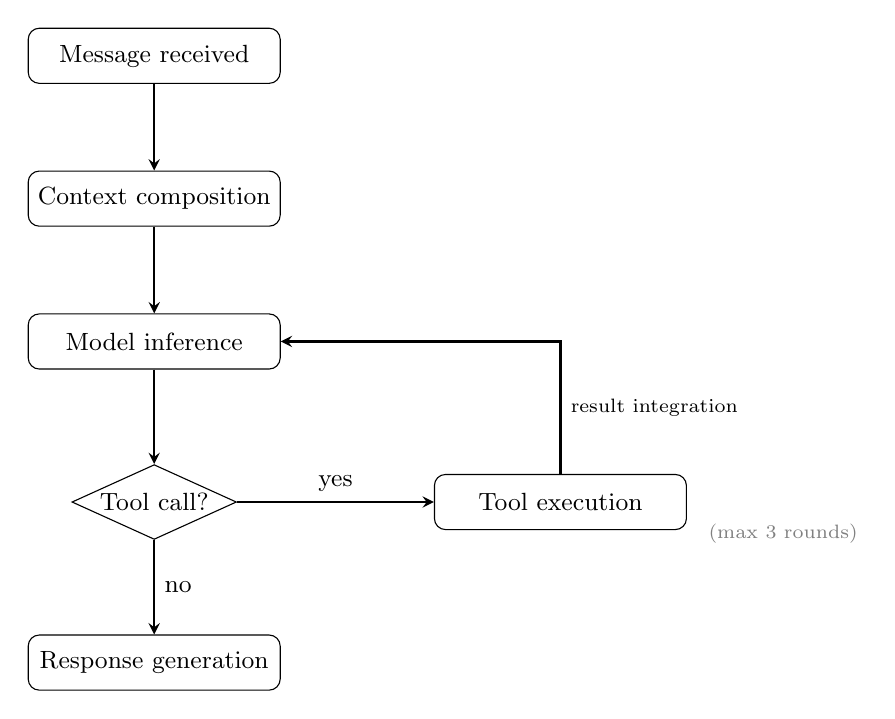
\begin{tikzpicture}[
    node distance=1.1cm and 2.5cm,
    box/.style={rectangle, draw, rounded corners, minimum width=3.2cm, minimum height=0.7cm, align=center, font=\small},
    decision/.style={diamond, draw, aspect=2.2, align=center, font=\small, inner sep=1pt},
    arrow/.style={->, >=stealth, thick},
    every node/.style={font=\small}
]
    \node[box] (msg) {Message received};
    \node[box, below=of msg] (ctx) {Context composition};
    \node[box, below=of ctx] (infer) {Model inference};
    \node[decision, below=1.2cm of infer] (decide) {Tool call?};
    \node[box, right=of decide] (exec) {Tool execution};
    \node[box, below=1.2cm of decide] (resp) {Response generation};

    \draw[arrow] (msg) -- (ctx);
    \draw[arrow] (ctx) -- (infer);
    \draw[arrow] (infer) -- (decide);
    \draw[arrow] (decide) -- node[above] {yes} (exec);
    \draw[arrow] (decide) -- node[right] {no} (resp);
    \draw[arrow] (exec) |- node[near start, right, font=\scriptsize] {result integration} (infer);

    % Loop limit annotation
    \node[font=\scriptsize, text=gray, right=0.15cm of exec, anchor=west, yshift=-0.4cm] {(max 3 rounds)};
\end{tikzpicture}
\caption{Tool execution flow for processing a student message. The system assembles context from the curriculum, learner model, conversation history, and tool schemas. The model may invoke tools (e.g.\ \texttt{record\_learning}, \texttt{advance\_topic}) whose results feed back into the next inference round, up to three rounds per turn.}
\label{fig:tool-flow}
\end{figure}

This multi-round architecture enables sequences that would be difficult to express in a single model output. For example, when a student submits an answer to a quiz question, the model might: (1) invoke \texttt{record\_learning} to evaluate the response, extract evidence, and apply confidence updates, and (2) if it judges the student ready, invoke \texttt{advance\_topic} to mark the current topic as completed and start the next one. All of this occurs within one conversational turn, with the final response summarising what happened and transitioning to the next activity.

To prevent excessive tool usage that could overwhelm the student or destabilise the conversation, the system enforces several constraints:

\begin{itemize}
\item \textbf{Maximum tools per turn}: At most three tool invocations per conversational turn.
\item \textbf{Quiz frequency}: At most one \texttt{quiz} invocation per curriculum node per session.
\item \textbf{Diagnostic limit}: At most one \texttt{create\_diagnostic} invocation per tutoring session.
\end{itemize}

These constraints are implemented as filters that remove disallowed tools from the available set based on current state, ensuring the model cannot invoke tools that would violate the limits.

\section{A Complete Tutoring Interaction}

To illustrate how these components interact, Appendix~\ref{appendix:walkthrough} presents a complete tutoring session in which a student learns about binary search trees. The session exercises all four phases of the system: intake (gathering goals and background via \texttt{ask\_student\_question}), diagnosis (identifying knowledge gaps via \texttt{create\_diagnostic}), plan generation (producing and negotiating a curriculum via \texttt{learning\_plan}), and iterative teaching with assessment (quizzing, updating confidence scores, resolving misconceptions, and advancing topics). The walkthrough demonstrates how the diminishing returns formula, misconception tracking, and user-initiated corrections operate in practice.

\section{Implementation Notes}

We implemented the system as a web application using Next.js for the application framework and React for the user interface. OpenRouter provides the language model integration, enabling access to multiple model providers through a unified API. This architecture allows experimentation with different underlying models without modifying the application code.

State management follows a three-tier structure for responsiveness and persistence. The first tier contains ephemeral state that exists only during the current session, such as which quiz question is currently displayed or whether a flashcard is showing its front or back. This state is managed in React component state and reconstructed from persistent data when the page loads.

The second tier contains message-level state that is persisted with each conversation message. This includes the tool outputs that generated interactive widgets, snapshots of the learner model at the time of each message, and records of curriculum changes. Storing this state with messages creates an immutable log that enables time-travel debugging and supports research analysis of tutoring trajectories.

The third tier contains chat-level state that represents the current status of the curriculum and learner model. This state is updated transactionally when tools execute and provides the authoritative source for display in the user interface. It persists across browser sessions through IndexedDB, enabling students to return to their learning progress after closing the application.

This local-first persistence strategy serves two purposes. It eliminates server dependencies, allowing the application to function offline and protecting student data privacy by keeping all information on the student's device. It also provides complete reproducibility for research purposes: the full trajectory of the tutoring session, including all tool invocations, learner model updates, and curriculum changes, can be reconstructed from the persisted state.

The language model's behaviour is governed by a system prompt that defines its pedagogical approach and tool usage guidelines. The prompt instructs the model to act as a Socratic tutor: asking before telling, scaffolding with fading support, normalising difficulty, and prioritising retrieval practice over passive re-explanation. It specifies when each tool is appropriate (e.g.\ use \texttt{quiz} for retrieval practice at topic boundaries, call \texttt{advance\_topic} when confidence exceeds approximately 80\% with demonstrated understanding) and when conversation alone suffices. The full system prompt is included in Appendix~\ref{appendix:prompt}.

The primary tutoring model is [MODEL NAME], selected for [REASON]. The automated evaluation uses [MODEL NAME] for the simulated student and [MODEL NAME] for the expert judge. We chose [cost-efficient / capable / etc.] models for the evaluation pipeline to enable [N] replications within budget constraints.

The implementation choices described here are not essential to the contribution of this thesis. The architectural principles of explicit representation, user editability, and tool-based pedagogy could be realized with different technology stacks. What matters is that the implementation faithfully instantiates these principles in a system suitable for experimental evaluation of the hypothesis that user-editable representations improve learning outcomes.

\chapter{Experimental Design}

The preceding chapters have established the theoretical motivation for user-editable representations in tutoring systems and described the architecture that instantiates these principles. The central claim of this thesis is that granting users control over explicit pedagogical representations improves learning outcomes compared to system-controlled, implicit representations. This chapter describes the experimental methodology designed to test this claim. The evaluation proceeds in two phases: an automated evaluation using simulated students that enables controlled comparison across experimental conditions, and a human study that captures how real learners experience and interact with the system. This chapter presents the design and methodology for both phases, with results reported in Chapter 6.

\section{Task Definition}

This section defines the tutoring task under evaluation. A precise task definition establishes which actions are available to the user, which actions the system performs, and what constitutes a single session. This framing distinguishes the task being solved from the specific solution we propose.

\subsection{Session Scope}

A tutoring session begins when a user arrives with a learning goal and ends when the user leaves or the learning goal is addressed. The user brings a topic they wish to learn, at any level of specificity. Goals may range from broad (``I want to understand recursion'') to narrow (``I need to solve this specific type of equation''). The system does not assume prior knowledge; it assesses the user's starting state through diagnostic questions.

A session is self-contained. The system does not retain information across sessions, and all state persists only within a single interaction. This scope matches the single-session evaluation design described in Section~\ref{sec:experimental-design}.

\subsection{User Actions}

The user can perform five types of actions during a session:

\begin{enumerate}
    \item \textbf{Converse}: Send messages to the tutor, ask questions, request explanations, and respond to prompts.
    \item \textbf{Answer assessments}: Respond to diagnostic questions and quizzes that the system presents.
    \item \textbf{View the curriculum}: Inspect the learning plan, including topics, prerequisites, and progress status.
    \item \textbf{Edit the curriculum}: Request modifications to the topic sequence, add or remove topics, or adjust prerequisites.
    \item \textbf{View and correct the learner model}: Inspect the system's confidence estimates for each topic, view the evidence underlying those estimates, and adjust scores the user believes are incorrect.
\end{enumerate}

Actions 1 and 2 are available in any conversational tutoring system. Actions 3 through 5 are the additions this work proposes to evaluate. The baseline condition restricts the user to actions 1, 2, and a read-only version of action 3.

\subsection{System Actions}

The system performs six types of actions:

\begin{enumerate}
    \item \textbf{Gather information}: Ask intake questions to understand the user's goals, constraints, and prior experience.
    \item \textbf{Diagnose prior knowledge}: Generate and administer diagnostic assessments to identify what the user already knows and where misconceptions exist.
    \item \textbf{Plan the curriculum}: Construct a sequence of topics with prerequisite relationships based on the user's goal and diagnostic results.
    \item \textbf{Teach}: Provide explanations, examples, and scaffolded instruction through conversation.
    \item \textbf{Assess understanding}: Pose questions to check comprehension, evaluate responses, and extract evidence of learning.
    \item \textbf{Update the learner model}: Adjust confidence estimates based on assessment results, user corrections, and observed interactions.
\end{enumerate}

These actions correspond to standard tutoring functions identified in the ITS literature. The system implements actions 1, 2, 3, 5, and 6 through discrete tools (Table~\ref{tab:tool-catalog}), while action 4 emerges from the language model's conversational generation.

\subsection{Relationship to the Research Question}

The research question asks whether adding user actions 4 and 5 (editing the curriculum and correcting the learner model) improves learning outcomes compared to a system that omits them. The task itself, tutoring a user toward a learning goal, remains constant across conditions. What varies is the set of actions available to the user.

This framing isolates the contribution under study. We do not compare different tutoring approaches or different system architectures. We compare the same task with and without two specific user capabilities.

\section{Evaluation Objectives}

The primary objective of this evaluation is to determine whether explicit, user-editable representations of the curriculum and learner model causally improve learning outcomes. The Background chapter established that classical Intelligent Tutoring Systems achieved educational effectiveness through structured representations, while Chapter 3 documented how contemporary LLM tutors have largely abandoned these structures in favour of conversational flexibility. The system described in Chapter 4 attempts to combine both approaches, but the mere existence of explicit representations does not guarantee they benefit learning. Users might ignore the curriculum graph entirely, or the cognitive overhead of managing their own learner model might distract from the learning task itself.

To address these possibilities, the evaluation must isolate the effects of each component. Simply comparing the full system against a baseline tutor would reveal whether the combination of features improves outcomes, but it would not identify which features contribute to any observed effect. A student might benefit primarily from seeing their mastery trajectory visualised, with the curriculum structure providing little additional value, or vice versa. Understanding which components matter, and whether they interact synergistically, is essential for guiding future system design.

This evaluation prioritises measurable learning outcomes over user satisfaction. As documented in Chapter 3, existing evaluations of LLM tutoring systems have relied primarily on surveys asking whether users found the experience helpful or the content relevant \citep{chen2024chattutor}. While user experience matters, it does not directly address whether learning occurred. A student might report high satisfaction with a tutor that provides entertaining explanations without actually improving their understanding of the material. By measuring knowledge through pre-tests and post-tests administered before and after each tutoring session, this evaluation grounds its conclusions in demonstrated learning rather than self-reported impressions.

\section{Experimental Design: Factorial Ablation Study}
\label{sec:experimental-design}

The experimental design employs a two-by-two factorial structure that systematically varies the visibility and editability of the two primary representations: the curriculum plan and the learner model. This factorial approach enables both main effect analysis, determining whether each component independently contributes to learning, and interaction analysis, determining whether the components work together synergistically.

\subsection{Experimental Conditions}

The four experimental conditions correspond to the cells of the two-by-two design. The first factor controls whether the curriculum plan is visible and editable by the student. When enabled, students can see the directed acyclic graph of topics, understand prerequisite relationships, and request modifications to the structure. When disabled, the system still maintains an internal curriculum but does not expose it to the user, operating more like a standard conversational agent.

The second factor controls whether the structured learner model is visible and editable. When enabled, students can inspect their mastery confidence for each topic, view the evidence that contributed to these estimates, and adjust scores they believe are incorrect. When disabled, the system maintains mastery tracking internally but presents only narrative summaries of progress, similar to the Learning Profile approach used in ChatTutor \citep{chen2024chattutor}.

The full system condition enables both the curriculum and learner model, instantiating the complete architecture described in Chapter 4. Students in this condition can see and edit the topic graph, inspect and adjust their mastery estimates, and observe how their progress relates to the curriculum structure. This condition tests the central hypothesis that user control over explicit representations improves learning.

The plan-only condition enables the curriculum but hides the structured learner model. Students can see and modify the topic sequence but cannot inspect their mastery confidence or the evidence underlying the system's assessment of their knowledge. This condition isolates the contribution of curriculum visibility, testing whether seeing the learning path provides value independent of mastery transparency.

The model-only condition shows the curriculum as read-only but enables editing of the structured learner model. Students can see the topic graph and prerequisite relationships but cannot modify the plan structure. They can inspect and adjust their mastery estimates for each topic as it arises. This condition isolates the contribution of editable mastery tracking, testing whether learner control over self-assessment provides value beyond passive curriculum awareness.

The baseline condition makes the curriculum visible but read-only, and hides the structured learner model entirely. This configuration mirrors ChatTutor's architecture: their Course Design Tool generates a curriculum that students can view but not modify, and their Learning Profile is ``not directly presented to users'' \citep{chen2024chattutor}. Like ChatTutor, the baseline allows the system to autonomously restructure the curriculum during the session; the restriction is that the \textit{student} cannot initiate modifications. By replicating these design choices, the baseline represents the current state of the art in agentic LLM tutoring.

This design has an important implication for interpreting results. Because the curriculum is visible in all four conditions, the plan factor isolates the effect of \textit{negotiability} (editability). However, because the learner model is hidden in the baseline conditions, the model factor captures the combined effect of \textit{inspectability} (visibility) and \textit{negotiability} (editability). Table~\ref{tab:ablation-factors} clarifies what each experimental factor tests.

\begin{table}[ht]
\centering
\caption{What each experimental factor tests, given the baseline configuration.}
\label{tab:ablation-factors}
\begin{tabular}{lll}
\toprule
\textbf{Factor} & \textbf{Baseline state} & \textbf{What enabling tests} \\
\midrule
Plan editability & Visible, read-only & Negotiability alone \\
Model visibility+editability & Hidden & Inspectability + negotiability (combined) \\
\bottomrule
\end{tabular}
\end{table}

This asymmetry reflects the state of the art we compare against. ChatTutor already shows the curriculum, so testing visibility would compare against a straw man. ChatTutor hides the learner model, so our comparison captures the full contribution of making it explicit and editable. Section~\ref{sec:limitations} discusses how future work could disentangle inspectability from negotiability for the learner model by including a visible-but-read-only condition.

Table~\ref{tab:ablation-conditions} summarises the four conditions and their feature configurations.

\begin{table}[ht]
\centering
\caption{Experimental conditions in the factorial ablation study.}
\label{tab:ablation-conditions}
\begin{tabular}{lcccc}
\toprule
\textbf{Condition} & \textbf{Plan Visible} & \textbf{Plan Editable} & \textbf{Model Visible} & \textbf{Model Editable} \\
\midrule
Full System & \checkmark & \checkmark & \checkmark & \checkmark \\
Plan Only & \checkmark & \checkmark & \texttimes & \texttimes \\
Model Only & \checkmark & \texttimes & \checkmark & \checkmark \\
Baseline & \checkmark & \texttimes & \texttimes & \texttimes \\
\bottomrule
\end{tabular}
\end{table}

\subsection{Hypotheses}

The evaluation distinguishes between confirmatory and exploratory hypotheses to maintain statistical rigour while enabling broader investigation.

\textbf{Confirmatory hypothesis (H1):} The full system produces greater normalised learning gains than the baseline. This primary hypothesis tests whether adding curriculum negotiability and learner model inspectability/negotiability improves learning outcomes over the state-of-the-art configuration. The confirmatory test uses Welch's t-test at $\alpha = 0.05$.

\textbf{Exploratory hypotheses:} Four secondary hypotheses examine individual contributions. H2a compares full system against plan-only to test whether learner model inspectability and negotiability contribute beyond curriculum negotiability alone; this comparison primarily targets the structured adaptation mechanism (mastery visibility enables better pacing) and error correction of mastery estimates. H2b compares full system against model-only to test whether curriculum negotiability contributes beyond learner model inspectability and negotiability; this targets the error correction mechanism (students can skip mastered material) and user agency (students direct their learning path). H3a compares plan-only versus baseline to isolate the effect of curriculum negotiability, testing error correction and user agency. H3b compares model-only versus baseline to test the combined effect of learner model inspectability and negotiability, targeting structured adaptation and error correction of mastery estimates. These comparisons use Welch's t-tests without multiple comparison correction, consistent with their exploratory framing.

Note that H3a provides a clean test of negotiability (since visibility is constant), while H3b tests inspectability and negotiability together (since the baseline hides the learner model). This asymmetry limits our ability to attribute effects specifically to inspectability or negotiability for the learner model, a limitation we address in Section~\ref{sec:limitations}.

\textbf{Interaction effects (H4):} The factorial design enables analysis of whether the benefit of one component depends on the presence of the other. A 2-way ANOVA tests main effects of plan visibility and model visibility, plus their interaction. A positive interaction would indicate synergy; negative interaction would suggest diminishing returns from combining the features.

\section{Automated Evaluation Methodology}

Before conducting studies with human participants, an automated evaluation using simulated students provides several advantages. It enables rapid iteration on the experimental protocol, identifies potential issues with scenario design or measurement instruments, and generates preliminary effect size estimates that inform sample size planning for the human study. Perhaps most importantly, automated evaluation provides perfect experimental control: the simulated student's knowledge state is known precisely, eliminating individual differences in prior knowledge that would otherwise introduce variance.

The automated evaluation involves running complete tutoring sessions with a language model that simulates student behaviour according to a specified persona and knowledge state. Each session follows a fixed protocol: a pre-test establishes baseline knowledge, the tutoring interaction proceeds for a specified number of turns, and a post-test measures knowledge after instruction. By comparing pre-test and post-test scores across experimental conditions, the evaluation estimates the learning gains attributable to each system configuration.

\subsection{Evaluation Scenarios}

The evaluation employs four scenarios spanning different academic domains and difficulty levels. Each defines a learning goal, curriculum structure, student persona, and assessment instruments. Selecting diverse scenarios reduces the risk that findings are specific to a particular domain or student type. Table~\ref{tab:scenarios} summarises the scenarios.

\begin{table}[ht]
\centering
\caption{Evaluation scenarios for automated assessment.}
\label{tab:scenarios}
\begin{tabular}{lllcp{4.5cm}}
\toprule
\textbf{Scenario} & \textbf{Domain} & \textbf{Level} & \textbf{Topics} & \textbf{Persona} \\
\midrule
Linear Equations & Algebra & Beginner & 4 & Anxious; prefers step-by-step guidance \\
Differentiation & Calculus & Intermediate & 6 & Struggles with abstraction; learns from examples \\
Python Debugging & CS & Beginner & 4 & Curious; eager to understand why errors occur \\
Bayes' Rule & Statistics & Intermediate & 5 & Overconfident; answers quickly \\
\bottomrule
\end{tabular}
\end{table}

Each scenario includes success criteria that define what constitutes effective tutoring and inform the expert judge evaluation described in Section~\ref{sec:expert-judge}.

\subsection{Knowledge Gap Modelling}

A critical challenge in automated evaluation is ensuring that the simulated student exhibits realistic learning behaviour. If the student begins the session already knowing the material, there is no opportunity to measure learning gains. If the student cannot learn at all, improvements in tutoring quality cannot produce measurable effects. The evaluation addresses this challenge through explicit knowledge gap modelling.

Each scenario defines knowledge gaps that specify which topics the simulated student does not initially understand. A knowledge gap comprises a topic identifier, an error rate between zero and one representing the probability of answering incorrectly on that topic, and optionally a misconception describing what the student wrongly believes. For example, in the linear equations scenario, the student has an error rate of 0.8 on two-step equations with the misconception that they often apply operations in the wrong order, dividing before subtracting.

These knowledge gaps serve two functions. During the pre-test, they calibrate the student's initial performance to a target level, typically around 40 to 60 percent correct. This creates room for measurable improvement while ensuring the student is not so uninformed that the tutoring task becomes trivial. During the tutoring session, the misconceptions guide the simulated student's responses, causing them to make realistic errors that the tutor must detect and address.

We designed the knowledge gaps so that topics early in the curriculum (those with fewer prerequisites) have lower error rates, while topics later in the sequence have higher error rates. This pattern reflects realistic learning trajectories where foundational concepts are more accessible than advanced applications that build upon them.

\subsection{Simulated Student Behaviour}

The simulated student is implemented as a language model operating under a persona prompt that specifies how to behave during the tutoring interaction. The persona prompt instructs the model to respond authentically and succinctly, to reference its understanding or confusion, to accept helpful guidance, to ask clarifying questions when needed, and to occasionally reflect on what it has learned. The prompt instructs the model to avoid meta-commentary about being an AI and to behave within the capabilities of a human student.

During the tutoring session, the simulator maintains a conversation history and generates responses based on the tutor's messages. When the tutor asks a question, the student responds according to its knowledge state and persona. An anxious student might express uncertainty even when their answer is correct, while an overconfident student might assert incorrect answers with unwarranted certainty.

\subsection{Pre-Test and Post-Test Protocol}

We measure learning gains through multiple-choice assessments administered before and after the tutoring session. Each scenario includes five pre-test questions and five post-test questions, with each question mapped to a specific topic in the curriculum. We designed the questions as isomorphic pairs: the pre-test and post-test assess the same underlying concept but use different surface features to prevent simple pattern matching.

For example, in the linear equations scenario, the pre-test asks ``Solve for x: x + 7 = 12'' while the post-test asks ``Solve for y: y - 9 = 15''. Both questions assess one-step equation solving, but the change in variable name, operation, and specific numbers prevents the student from memorising the answer during the session.

The pre-test employs a forced-error mechanism based on the knowledge gaps. When the simulated student encounters a question on a topic for which a knowledge gap is defined, a random draw against the error rate determines whether the student is forced to answer incorrectly. If the error rate is 0.8 and the random draw falls below this threshold, the student receives instructions to answer based on their misconception rather than their best guess. This mechanism ensures that pre-test scores reflect the defined knowledge state rather than lucky guesses.

The forced-error mechanism manufactures predetermined scores rather than simulating genuine knowledge. This is a deliberate choice to standardise starting conditions across experimental groups, ensuring that observed learning gain differences reflect tutoring effectiveness rather than pre-test variance. The limitation is that pre-test scores lack ecological validity as knowledge assessments.

The post-test employs an evidence gating mechanism that validates whether learning actually occurred during the session. For questions targeting knowledge gap topics, the simulated student must produce a JSON response containing both an answer and a verbatim evidence quote from the tutoring transcript. The system then verifies this evidence through two checks: a fuzzy token overlap test that confirms at least 60\% of meaningful tokens in the quote appear in the transcript (accounting for paraphrasing), and a keyword relevance test that confirms the quote contains at least one topic-specific keyword (preventing false positives from generic transcript text). If both checks pass, the student's answer is trusted. If either check fails---or if the student cannot provide valid JSON---the answer is forced to a misconception-aligned distractor, a predetermined wrong answer that reflects the student's original misconception for that topic. Each knowledge gap specifies this distractor index; when none is configured, the first wrong option serves as a fallback. This evidence gating mechanism prevents attributing learning gains to topics that were never addressed and addresses the ceiling effect where the LLM student could otherwise answer correctly based on parametric knowledge rather than tutoring content.

The primary outcome metric is normalised learning gain \citep{hake1998interactive}, calculated as the post-test score minus the pre-test score divided by the maximum possible improvement from the pre-test score:
\begin{equation}
g = \frac{\text{post} - \text{pre}}{100 - \text{pre}}
\end{equation}
This normalisation accounts for differences in pre-test performance across conditions. A student who scores 80\% on the pre-test has less room for improvement than one who scores 40\%, so raw gain would be misleading. Normalised gain expresses improvement as a fraction of possible improvement, enabling fair comparison across different starting points.

\subsection{Limitations of Automated Evaluation}

The automated evaluation methodology offers experimental control but has important limitations that must be acknowledged. Most significantly, using an LLM to simulate learning from an LLM tutor, then using another LLM to judge quality, creates a closed evaluation loop with potentially shared biases. If the tutor and simulated student share similar linguistic patterns or reasoning approaches, the tutor may appear more effective than it would with real learners who process information differently.

The simulated student also lacks ecological validity. Real students exhibit working memory constraints, attention lapses, emotional responses to failure, and motivational fluctuations that affect learning. A simulated student that can perfectly recall the conversation transcript does not experience the cognitive load that makes learning difficult.

The post-test mechanism measures whether topics were covered in the transcript, not whether learning occurred in any meaningful sense. Real learning involves encoding, consolidation, and retrieval from long-term memory. The simulated student's transcript-based responses test context window retrieval, which is fundamentally different from the knowledge transfer that education aims to produce.

For these reasons, the automated evaluation should be understood as hypothesis-generating rather than hypothesis-confirming. It identifies promising patterns and estimates effect sizes, but the human study described in Section~\ref{sec:human-study} complements these findings by capturing how real learners perceive and interact with the system.

\subsection{Automated Quality Assessment}
\label{sec:expert-judge}

Pre-test and post-test scores measure whether learning occurred, but they do not directly assess the quality of the tutoring process. A tutor might achieve learning gains through inefficient methods, excessive quizzing, or poor scaffolding that happens to work despite its flaws. To assess pedagogical quality, each tutoring session is evaluated using an LLM-as-judge approach \citep{zheng2023judging}, where a language model applies a structured rubric to rate session transcripts.

The assessment receives the scenario context including the learning goal, student persona, success criteria, and the student's known knowledge gaps, along with the complete session transcript. It evaluates the tutor on five dimensions, each scored from zero to one, with a weighted overall score. These dimensions draw on established frameworks for characterising effective tutoring, particularly the ICAP framework's emphasis on active and constructive learning \citep{chi2014icap}. Time allocation efficiency (weight 0.25) assesses whether the tutor prioritised weak areas and moved quickly past mastered material. Diagnostic accuracy (weight 0.20) assesses whether the tutor identified student misconceptions and addressed each with targeted corrections. Scaffolding quality (weight 0.20) assesses whether the tutor progressed from simple to complex content with appropriate hints that faded as understanding grew. Gap coverage depth (weight 0.25) assesses whether knowledge gap topics received thorough explanation, practice, and verification. Communication style (weight 0.10) assesses warmth, clarity, and encouragement; this dimension serves as a control that should remain stable across conditions since it reflects the tutor model rather than the experimental manipulation.

The assessment also provides qualitative feedback including notes on tool usage, whether the tutor advanced topics before the student demonstrated adequate understanding, a list of strengths, and suggestions for improvement. This qualitative feedback supports analysis of tutoring patterns beyond what numerical scores capture.

This automated assessment has not been calibrated against human expert ratings, which limits confidence in its validity. If the tutor and judge share similar model architectures or training data, the judge may rate highly whatever patterns the tutor produces, regardless of actual pedagogical quality. The assessment scores should therefore be interpreted as consistency metrics that may identify relative differences between conditions, rather than as ground-truth measures of teaching quality. Prior work has shown that strong LLM judges can achieve approximately 80\% agreement with human evaluators, comparable to inter-annotator agreement among humans, though these judges also exhibit systematic biases including position bias, verbosity bias, and self-enhancement bias when rating outputs from their own model family \citep{zheng2023judging, chen2024judgementbias}.

\section{Metrics and Measurements}

The evaluation collects multiple metrics that together characterise the effectiveness and behaviour of each experimental condition. The primary outcome is normalised learning gain as described above. Secondary outcomes capture aspects of the tutoring process that may explain observed learning differences.

We record tool usage as a count of each tool invocation during the session. High usage of the quiz tool might indicate excessive testing, while high usage of the plan update tool might indicate responsive adaptation to student needs. Comparing tool usage patterns across conditions reveals how the availability of explicit representations changes tutoring behaviour. In particular, \texttt{advance\_topic} calls are tracked separately as a mechanism metric: in plan-editable conditions, student-directed advancement represents plan agency, while in non-editable conditions, it reflects tutor-autonomous progression.

Edit events track when students exercise control over the representations. A plan modification occurs when the student requests changes to the curriculum structure, such as removing a topic they already know or adding a prerequisite they need to review. A mastery override occurs when the student adjusts their confidence score, indicating disagreement with the system's assessment. These events are only possible in conditions where the relevant representation is editable, but their frequency in those conditions indicates how actively students engage with the control mechanisms.

The mastery trajectory records the average confidence across all curriculum nodes at each turn of the conversation. Plotting this trajectory reveals the pace of learning and whether confidence grows steadily or in bursts following key insights. Comparing trajectories across conditions may reveal different learning dynamics associated with different feature configurations.

\subsection{Statistical Analysis Plan}

The confirmatory hypothesis (Full vs Baseline) is tested using Welch's t-test, which accommodates unequal variances between groups. The test uses $\alpha = 0.05$ with a two-tailed alternative. Effect sizes are reported as Cohen's d with conventional thresholds \citep{cohen1988power}: below 0.2 negligible, 0.2--0.5 small, 0.5--0.8 medium, above 0.8 large. All pairwise comparisons report 95\% confidence intervals for the mean difference.

Exploratory pairwise comparisons also use Welch's t-tests. Holm--Bonferroni step-down correction \citep{holm1979simple} is applied separately to three families of comparisons---overall normalised gain, gap-only normalised gain, and judge quality scores---to control the family-wise error rate while preserving more statistical power than the classical Bonferroni correction. Both raw and adjusted p-values are reported.

For the factorial design, a 2-way ANOVA tests main effects of plan editability and learner model editability, plus their interaction. This provides F-statistics and p-values for each factor independently, complementing the pairwise comparisons. Effect sizes for ANOVA effects are reported as partial eta-squared ($\eta^2_p = \text{SS}_{\text{effect}} / (\text{SS}_{\text{effect}} + \text{SS}_{\text{residual}})$), with conventional thresholds: below 0.01 negligible, 0.01--0.06 small, 0.06--0.14 medium, above 0.14 large. The interaction term directly addresses whether the two features combine synergistically or redundantly.

\subsection{Sample Size Justification}

Power analysis targets 80\% power \citep{cohen1988power} to detect a medium effect ($d = 0.5$) at $\alpha = 0.05$. For a two-sample t-test under these parameters, approximately 64 observations per group are required. The automated evaluation runs 20 replications per condition-scenario cell across 4 scenarios, yielding 80 observations per condition (320 total runs). This exceeds the minimum required sample size while remaining within computational budget constraints (approximately \$6--7 for the full study using cost-efficient models).

\section{Threats to Validity}

Several threats to validity must be acknowledged. Internal validity is threatened by the automated evaluation's circularity: if the tutor, simulated student, and judge share similar model architectures, observed effects may reflect model-specific patterns rather than genuine pedagogical differences. The forced-error mechanism in pre-tests further limits internal validity since it manufactures starting conditions rather than measuring them. The judge evaluator receives the full tutoring transcript, which implicitly contains information about tool availability---for example, only plan-editable conditions can produce plan restructuring events in the transcript. Although the judge prompt instructs evaluation based solely on pedagogical quality, this transcript-to-judge leakage could introduce systematic bias.

The \texttt{parseAnswer} fallback deserves mention: when the simulated student produces an unparseable response, the system selects a random answer. This fallback uses a seeded random number generator keyed to the run identifier and question identifier, ensuring reproducibility across repeated evaluations. Without seeding, non-deterministic fallback behaviour would introduce uncontrolled variance.

External validity is limited by scenario selection. All four scenarios cover STEM domains where knowledge structures are relatively well-defined. The system's effectiveness in humanities or domains requiring subjective judgment remains untested. The simulated student personas, while varied, may not capture the full range of real learner characteristics.

Construct validity concerns whether the measurements capture the intended constructs. Normalised learning gain in the automated evaluation measures transcript coverage rather than knowledge transfer. The quality assessment dimensions, while grounded in the ICAP framework, have not been validated against human expert judgments. With six pairwise comparisons conducted across three outcome families (overall gain, gap gain, judge score), multiple comparisons inflate the family-wise Type~I error rate. Holm--Bonferroni correction is applied to control this, though the exploratory nature of the factorial analysis means that significant results should be interpreted as hypothesis-generating rather than confirmatory. The human study complements these automated measures by capturing perceived learning, control, and trust from real participants, though it does not independently measure knowledge acquisition.

\section{Human Study Protocol}
\label{sec:human-study}

The automated evaluation estimates learning gains under controlled conditions, but simulated students cannot capture how real learners experience the system. Real users face cognitive load when managing an explicit learner model while trying to learn new material. They may ignore the curriculum graph, feel overwhelmed by the additional interface, or find the transparency genuinely helpful in ways that a simulated persona cannot express. The human study addresses these questions by observing real participants as they use both system configurations in supervised sessions.

The human study does not measure learning gains. With approximately ten participants and a single 15-minute session per condition, the study lacks statistical power to detect meaningful differences in knowledge acquisition. Instead, it focuses on user experience: whether participants perceive greater control and transparency when using the full system, whether the editable representations increase or undermine trust, and whether participants actually engage with the editing capabilities. These questions cannot be answered by the automated evaluation regardless of sample size.

\subsection{Study Design}

The study uses a within-subjects design comparing two conditions. In the baseline condition, participants interact with a conversational tutor that displays the curriculum as a read-only plan but hides the structured learner model. In the full system condition, participants can additionally edit the curriculum plan and inspect and adjust their learner model, including mastery confidence scores and evidence logs. These conditions correspond to the baseline and full system conditions from the factorial design in Section~\ref{sec:experimental-design}.

A within-subjects design was chosen over a between-subjects comparison for two reasons. First, each participant directly experiences both configurations, yielding richer qualitative data about perceived differences. Second, individual differences in learning style, prior knowledge, and technology familiarity are controlled because each participant serves as their own control. The tradeoff is potential order effects, which the counterbalancing scheme below mitigates.

A full 2$\times$2 factorial was not feasible for the human study. Distributing ten participants across four conditions would yield two to three per cell, insufficient for any analysis. The A/B comparison between baseline and full system tests the primary hypothesis (H1) directly and maximises statistical power within the available sample.

\subsection{Topics and Counterbalancing}

Each participant uses both systems, each with a different learning topic. Two topics were selected to fall outside the typical informatics curriculum, minimising the chance that prior knowledge confounds comparisons: quantum entanglement and CRISPR gene editing. Both are accessible to non-specialists, conceptually rich enough for a 15-minute session, and roughly equivalent in complexity.

Using different topics for each system prevents a carryover confound: if participants studied the same topic twice, knowledge gained in the first session would inflate performance in the second, regardless of which system was used. The two-topic design ensures that differences between conditions reflect the system configuration rather than accumulated knowledge.

A Latin square counterbalancing scheme cycles every four participants, varying both system order and topic assignment. Table~\ref{tab:counterbalancing} shows the rotation.

\begin{table}[ht]
\centering
\caption{Counterbalancing matrix for the human study. The pattern repeats every four participants.}
\label{tab:counterbalancing}
\begin{tabular}{cllll}
\toprule
\textbf{Group} & \textbf{First System} & \textbf{First Topic} & \textbf{Second System} & \textbf{Second Topic} \\
\midrule
1 & Baseline & Quantum Entanglement & Full System & CRISPR Gene Editing \\
2 & Baseline & CRISPR Gene Editing & Full System & Quantum Entanglement \\
3 & Full System & Quantum Entanglement & Baseline & CRISPR Gene Editing \\
4 & Full System & CRISPR Gene Editing & Baseline & Quantum Entanglement \\
\bottomrule
\end{tabular}
\end{table}

Participant $n$ is assigned to group $((n - 1) \bmod 4) + 1$. Across every four participants, each system appears equally often in first and second position, and each topic appears equally often with each system.

\subsection{Participants}

The target sample is approximately ten university students recruited through departmental mailing lists. No inclusion criteria beyond basic computer literacy are imposed, though participants are expected to be unfamiliar with both learning topics. The study received ethical approval from the university ethics committee. Participants are not financially compensated, consistent with university policy.

\subsection{Procedure}

Sessions are individual, supervised, and conducted in person on the researcher's laptop. Each session lasts approximately 45 minutes and follows the structure in Table~\ref{tab:procedure}.

\begin{table}[ht]
\centering
\caption{Session procedure for the human study.}
\label{tab:procedure}
\begin{tabular}{rp{10cm}}
\toprule
\textbf{Minutes} & \textbf{Activity} \\
\midrule
0--2 & Welcome and study explanation. The researcher explains the session structure and emphasises that honest feedback, including negative feedback, is valued. The researcher clarifies that the study evaluates the systems, not the participant. \\
2--3 & Consent. The researcher reviews anonymisation, data handling, and the right to withdraw at any time. \\
3--4 & Setup. The researcher configures the first system and topic per the counterbalancing matrix and provides the starting prompt. \\
4--19 & First system session (15 minutes). The participant interacts freely; the researcher intervenes only for technical issues. \\
19--22 & Per-system questionnaire for the first system. \\
22--23 & Transition and brief break. The researcher configures the second system and topic. \\
23--38 & Second system session (15 minutes). \\
38--41 & Per-system questionnaire for the second system. \\
41--45 & Comparative questionnaire, debrief, and participant questions. \\
\bottomrule
\end{tabular}
\end{table}

The researcher remains silent during tutoring sessions unless a technical problem prevents the participant from continuing. This non-interference protocol ensures that measured perceptions reflect the system's behaviour rather than researcher guidance.

\subsection{Measurement Instruments}

The study collects three types of data: structured questionnaire responses, qualitative feedback, and automated interaction logs.

\paragraph{Per-system questionnaire.} After each system session, participants rate five statements on a five-point Likert scale (1~=~Strongly Disagree to 5~=~Strongly Agree):

\begin{enumerate}
    \item ``I felt in control of my learning process.'' (perceived control)
    \item ``I understood what the system was doing and why.'' (transparency)
    \item ``I trusted the system to guide my learning effectively.'' (trust)
    \item ``I felt like I was learning effectively.'' (perceived learning)
    \item ``Using this system required a lot of mental effort.'' (cognitive load, reverse-scored)
\end{enumerate}

Items 1 and 2 address whether the transparency and control mechanisms achieve their intended purpose. Item 3 tests whether exposing system state builds trust. Item 4 captures perceived learning as a subjective complement to the automated evaluation's objective measures. Item 5 tests whether the additional interface complexity introduces cognitive overhead that could offset the benefits of transparency. Each questionnaire concludes with one open-ended question: ``Any immediate reactions to this system?''

\paragraph{Comparative questionnaire.} After both sessions, participants answer five open-ended questions in a funnel structure that moves from unprompted impressions to specific probes:

\begin{enumerate}
    \item ``Which system did you prefer for learning, and why?''
    \item ``What differences did you notice between the two systems?''
    \item ``One system let you modify the tutoring plan, while the other only let you view it. Did this matter to you? Why or why not?''
    \item ``One system showed you what it believed about your understanding of each topic. What did you think about that?''
    \item ``Would you use either of these systems for actual studying? How?''
\end{enumerate}

Questions 1 and 2 capture initial reactions before any framing. Questions 3 and 4 then probe the two differentiating features (plan editability and learner model visibility) directly. This ordering records unprompted impressions before directed questions could introduce bias toward either system.

\paragraph{Interaction logs.} The system records timestamped user actions: plan views, plan edits, learner model inspections, and mastery score adjustments. These logs contain no message text, preserving participant privacy while providing behavioural data on how participants engage with the editable representations. At the end of each session, participants may voluntarily copy their interaction traces into the study form.

All questionnaire responses are collected through Microsoft Forms. The researcher enters the participant identifier and condition assignment; the participant completes the remaining fields. Interaction trace fields are optional and placed immediately after each system session to minimise the delay between interaction and submission.

\subsection{Analysis Plan}

The small sample size makes this study exploratory rather than confirmatory. Quantitative analysis of Likert responses uses the Wilcoxon signed-rank test \citep{wilcoxon1945individual} for paired comparisons between conditions, appropriate for ordinal data in a within-subjects design. Effect sizes are reported as matched-pairs rank-biserial correlation $r$. With ten participants, only large effects ($r > 0.5$) are likely to reach statistical significance, so the analysis emphasises effect size estimates over p-values.

Qualitative analysis of open-ended responses follows the thematic analysis approach described by \citet{braun2006thematic}. The researcher codes responses to identify recurring themes related to control, transparency, trust, and cognitive load, then examines whether themes differ systematically between conditions. Interaction logs supplement self-report data with objective measures of feature engagement: whether participants opened the plan, made edits, or inspected the learner model, and how frequently.

The human study results are interpreted alongside the automated evaluation. Where both evaluations agree (for example, if the automated evaluation shows learning gains and participants report higher perceived learning), confidence in the findings strengthens. Where they diverge, the discrepancy itself warrants discussion in Chapter~7.


\chapter{Results}

\chapter{Discussion}

The results presented in Chapter 6 provide evidence regarding the central hypothesis: that granting users transparency over and control of explicit pedagogical representations improves learning outcomes. This chapter interprets those results, connects them to the theoretical framework established in the Introduction, compares them to prior work, and draws implications for the design of future tutoring systems.

\section{Summary of Findings}

[To be written after Chapter 6 is complete. Structure: state the headline result for H1 (full system vs baseline). Then report the exploratory findings: H2a (full vs plan-only), H2b (full vs model-only), H3a (plan-only vs baseline), H3b (model-only vs baseline). Report the ANOVA interaction effect. Summarise the human study findings in a separate paragraph: Likert comparisons, qualitative themes, and feature engagement rates from interaction logs. Note where the two evaluation phases agree and where they diverge.]

\section{Interpreting the Three Mechanisms}

The Introduction proposed three mechanisms through which inspectability and negotiability improve learning: error correction, structured adaptation, and user agency. This section examines each mechanism against the evidence.

\subsection{Error Correction}

[To be written. Interpret whether plan edits and mastery overrides occurred and whether they correlated with learning gains. Key data sources: edit event counts from the automated evaluation (how often did the simulated student or real participants modify the curriculum or adjust mastery scores?), H3a results (plan editability vs baseline, which primarily tests this mechanism), and qualitative reports from the human study (did participants describe correcting the system?). If plan edits were rare, discuss whether the curriculum generation was accurate enough to make correction unnecessary, or whether participants did not understand the editing capability.]

\subsection{Structured Adaptation}

[To be written. Interpret whether mastery visibility changed tutoring dynamics. Key data sources: mastery trajectory plots across conditions (did conditions with visible learner models show different confidence growth patterns?), H3b results (model visibility+editability vs baseline, which targets this mechanism), and the expert judge's scaffolding quality scores. If the tutor made better advancement decisions when the learner model was visible, this supports the structured adaptation mechanism. If not, consider whether the LLM's conversational inference already provides sufficient signal without explicit mastery tracking.]

\subsection{User Agency}

[To be written. Interpret whether participants who could edit representations reported greater perceived control and learning. Key data sources: Likert items 1 (``I felt in control of my learning process'') and 4 (``I felt like I was learning effectively'') from the human study, qualitative responses to comparative questions 1 and 2 (unprompted preferences and noticed differences), and interaction log data on feature engagement. If participants engaged with editing but did not report greater control, consider whether the interface design failed to communicate the available agency.]

\section{Comparison with Related Work}

[To be written. Compare findings to three bodies of prior work:

(1) The Open Learner Model literature reported mixed results on editable models, with effectiveness depending on learner characteristics and visualisation quality \citep{hooshyar2020olm}. Do our results replicate this pattern? Did certain participant profiles benefit more from editability than others?

(2) ChatTutor's evaluation focused on satisfaction and stability rather than learning gains \citep{chen2024chattutor}. Our automated evaluation measures learning gains directly. How do our baseline results (which replicate ChatTutor's architecture) compare to our experimental conditions? Does the addition of editability and visibility produce measurable learning differences that satisfaction surveys would miss?

(3) Classical ITS evaluations demonstrated medium to large effect sizes for structured tutoring \citep{kulik2016itsmeta}. Where do our effect sizes fall relative to this benchmark? If smaller, discuss whether the single-session scope or the automated evaluation methodology accounts for the difference.]

\section{Design Implications}

[To be written. Based on the results, what should designers of future LLM tutoring systems take away?

Consider addressing: (1) When is transparency worth the engineering cost? If the learner model factor shows a positive effect, the investment in explicit mastery tracking is justified. If not, simpler architectures may suffice. (2) When might editability hurt rather than help? If cognitive load scores (Likert item 5) were higher in the full system condition, the additional interface complexity may offset the benefits of control. (3) What is the minimum viable transparency? If plan visibility alone (which all conditions share) accounts for most of the benefit, the additional cost of editable representations may not be justified for all contexts. (4) How do these findings apply beyond STEM domains?]

\section{Limitations}
\label{sec:limitations}

Several limitations qualify the conclusions of this work.

\textbf{Confounded factors for the learner model.} The experimental design tests curriculum negotiability in isolation (since the curriculum is visible in all conditions) but tests learner model inspectability and negotiability together (since the baseline hides the learner model). If the learner model factor shows a positive effect, we cannot determine whether the benefit arises from users seeing their mastery estimates, from users correcting inaccurate estimates, or from both. A future study could disentangle these factors by including a condition where the learner model is visible but read-only. We did not include this condition because it does not correspond to any existing system (ChatTutor hides the learner model entirely), and our primary goal was to compare against the state of the art rather than to isolate every possible factor.

\textbf{Automated evaluation circularity.} The automated evaluation uses an LLM to simulate learning from an LLM tutor, then uses another LLM to judge quality. This creates a closed loop with potentially shared biases. If the tutor and simulated student share similar linguistic patterns, the tutor may appear more effective than it would with real learners. The human study breaks this loop by placing real participants in front of the system, though its small sample and focus on perceived experience rather than measured learning gains limit the extent to which it can confirm the automated findings.

\textbf{Domain specificity.} All evaluation scenarios cover STEM domains where knowledge structures are well-defined and prerequisite relationships are clear. The system's effectiveness in humanities or domains requiring subjective judgment remains untested.

\chapter{Conclusions}

This thesis investigated whether granting users transparency over and control of explicit pedagogical representations improves learning outcomes in LLM-based tutoring. This chapter summarises the contributions, identifies directions for future work, and offers closing reflections.

\section{Summary of Contributions}

This work made four contributions.

First, we presented a design framework for user-editable pedagogical representations, defining how curriculum graphs and learner models serve as shared interfaces between human and machine. The framework operationalises the Open Learner Model principles of inspectability and negotiability \citep{bull2007invite, kay2013scrutability} within an LLM tutoring architecture, extending them from the learner model to the curriculum structure itself.

Second, we proposed an evaluation methodology focused on learning outcomes through pre- and post-tests, addressing the gap identified in Chapter 3 where existing LLM tutoring evaluations relied primarily on satisfaction surveys \citep{chen2024chattutor}. The factorial ablation design enables isolation of individual feature contributions rather than testing the system as a monolithic whole.

Third, we provided a reference implementation demonstrating that explicit state management, tool-based pedagogy, and conversational flexibility can coexist within a single architecture. The system maintains structured curriculum graphs and quantified mastery records while preserving the natural language fluency of the underlying language model.

Fourth, we conducted experimental evaluation comparing this approach against a baseline that mirrors the current state of the art in agentic LLM tutoring. [Add 1--2 sentences summarising the headline result once Chapter 6 is complete. E.g.: ``The results indicate that [finding], with [effect size] for the primary comparison.'']

\section{Future Work}

Several directions emerge from this work.

\textbf{Disentangling inspectability from negotiability.} The experimental design tests the learner model's inspectability and negotiability together. A future study could include a visible-but-read-only learner model condition to determine whether seeing mastery estimates is sufficient or whether the ability to correct them is what drives any observed benefit.

\textbf{Longitudinal evaluation.} This work evaluated single-session tutoring. Multi-session studies would reveal whether explicit representations support long-term knowledge retention and whether students continue to engage with editing capabilities over time or revert to passive use.

\textbf{Domain generalisation.} All evaluation scenarios covered STEM domains with well-defined prerequisite structures. Extending the approach to humanities, social sciences, or creative domains would test whether the curriculum graph representation generalises to less hierarchical knowledge structures.

\textbf{Adaptive transparency.} Rather than offering full editability to all users, future systems could adapt the level of transparency to the learner's expertise and preferences. Novice learners might benefit from a simplified view, while advanced learners might engage more productively with full control.

\textbf{Principled mastery estimation.} The current confidence update formula uses heuristic weights. Future work could replace this with a calibrated approach, such as Bayesian Knowledge Tracing adapted for natural language evidence, provided the resulting estimates remain interpretable enough to support the Open Learner Model principle.

[Add any additional future work directions that emerge from the results discussion.]

\section{Closing Remarks}

[To be written. 2--3 sentences that connect back to the opening motivation. The thesis began with the observation that LLM tutors operate as black boxes. Reflect on what the results say about whether opening that box matters for learning.]

% \bibliographystyle{plain}
\bibliographystyle{plainnat}
\bibliography{mybibfile}


% You may delete everything from \appendix up to \end{document} if you don't need it.
\appendix

\chapter{Complete Tutoring Interaction Walkthrough}
\label{appendix:walkthrough}

This appendix provides the full worked example summarised in Chapter 4, demonstrating how a tutoring session exercises curriculum generation, learner model tracking, and tool-based pedagogy.

\section{Intake Phase}

The tutor begins by invoking \texttt{ask\_student\_question} to gather essential information through a structured questionnaire. It presents four questions:

\begin{enumerate}
\item \textbf{Background}: What is your experience with data structures? (Options: No experience, Basic arrays/lists, Comfortable with recursion, Strong foundation)
\item \textbf{Goal focus}: What aspects of binary search trees matter most for your exam? (Options: Conceptual understanding, Implementation, Time complexity analysis, All of the above)
\item \textbf{Timeline}: When is your exam? (Options: This week, In 1-2 weeks, In 3-4 weeks, No deadline)
\item \textbf{Prior exposure}: Have you encountered BSTs before? (Options: Never, Briefly in lecture, Used them before, Implemented them)
\end{enumerate}

The student selects ``Basic arrays/lists'' for background (indicating uncertainty about recursion), ``Implementation'' for focus, ``In 1-2 weeks'' for timeline, and ``Briefly in lecture'' for prior exposure. The tool returns these structured responses, which the model uses to inform subsequent decisions.

\section{Diagnostic Phase}

Based on the intake revealing uncertainty about recursion, a prerequisite for understanding tree operations, the tutor invokes \texttt{create\_diagnostic} to generate five questions covering linked list traversal, recursive function tracing, tree terminology, and basic algorithmic thinking. The student answers four questions correctly but selects the wrong answer for recursive function tracing. The system invokes \texttt{record\_learning} to initialise confidence scores:

\begin{itemize}
\item \textbf{Basic data structures}: 0.65 confidence (correct diagnostic responses)
\item \textbf{Recursion}: 0.30 confidence (incorrect diagnostic response plus expressed uncertainty)
\item \textbf{Tree terminology}: 0.55 confidence (correct but minimal demonstration)
\end{itemize}

\section{Plan Generation Phase}

The tutor now invokes \texttt{learning\_plan} with the accumulated context. Given the goal, diagnostic results, timeline, and implementation focus, it produces a curriculum with six nodes:

\begin{enumerate}
\item \textbf{Recursion Fundamentals} (prerequisites: none, status: in\_progress)
\item \textbf{Tree Terminology and Traversal} (prerequisites: [1])
\item \textbf{BST Property and Search} (prerequisites: [2])
\item \textbf{BST Insertion} (prerequisites: [3])
\item \textbf{BST Deletion} (prerequisites: [4])
\item \textbf{Balanced Trees Overview} (prerequisites: [1,2,3,4,5])
\end{enumerate}

The tool output includes \texttt{requiresConfirmation: true}, so the system presents this curriculum to the student with the message: ``Based on your diagnostic results, I recommend starting with a recursion review since tree operations rely heavily on recursive thinking. Does this plan work for you?''

The student examines the plan and notes that balanced trees are not covered on their exam. They type: ``Can we remove the balanced trees topic?'' The tutor invokes \texttt{learning\_plan} to delete node 6, producing a five-topic curriculum. The confirmation message explains: ``Removed Balanced Trees Overview since it's not needed for your exam. This focuses your study on the core BST operations.'' The student approves the modified plan.

\section{Teaching and Assessment Phase}

Teaching begins on the recursion fundamentals topic. The tutor explains recursive thinking through the lens of tree operations, since this connects the review to the student's goal. It presents the concept of a base case using tree examples: ``Just as a recursive function needs a base case to stop, tree recursion naturally terminates at leaf nodes, which have no children.''

After the explanation, the tutor invokes \texttt{quiz} to check understanding with a question about base cases in recursive tree traversal. The student answers correctly. The model invokes \texttt{record\_learning} with evidence type \texttt{correct\_answer} and weight 0.4. The diminishing returns formula updates confidence:

\[
C_{\text{new}} = 0.30 + 0.4 \times (1 - 0.30) = 0.30 + 0.28 = 0.58
\]

The student answers a second question correctly, raising confidence to approximately 0.68. On the third question about what happens when a base case is missing, the student selects ``The function returns 0'' rather than the correct answer ``Infinite recursion / stack overflow.'' The model logs an incorrect response and records a misconception: the student believes a missing base case returns a default value rather than causing infinite recursion. Confidence decreases to approximately 0.52.

\section{Misconception Resolution}

The tutor addresses the misconception directly in its natural language response: ``When a base case is missing, the function keeps calling itself forever. Let me show you what happens step by step...'' It provides a concrete trace showing stack frames accumulating without termination.

The tutor then invokes \texttt{quiz} again with two questions focused specifically on base case behaviour. The student answers both correctly, demonstrating understanding of when and why recursion terminates. For each correct answer, the model invokes \texttt{record\_learning}. After the second correct answer:

\[
C_{\text{new}} = 0.62 + 0.35 \times (1 - 0.62) = 0.62 + 0.13 = 0.75
\]

With confidence above 0.70 and the misconception resolved (subsequent responses demonstrate correct understanding), the model judges the student ready to advance. It invokes \texttt{advance\_topic} to mark the recursion fundamentals node as completed and start tree terminology and traversal. The curriculum visualisation updates to show the first node with a completion indicator and the second node highlighted as the current focus.

\section{Progression Through the Curriculum}

This cycle continues through subsequent topics. When the student reaches BST insertion and correctly implements an insert function on the first attempt, the high-quality response produces evidence with weight 0.5, and confidence rises rapidly. When the student struggles with BST deletion, which involves the complex case of removing a node with two children, the model detects difficulty through incorrect answers and hint requests. It logs evidence with lower weights, causing confidence to grow more slowly. The tutor provides additional scaffolding, breaking down the in-order successor approach into smaller steps before the student demonstrates mastery.

\section{User Inspection and Correction}

Throughout this process, the student can inspect the learner model to understand the system's beliefs. Clicking on the ``Recursion Fundamentals'' node reveals:

\begin{itemize}
\item \textbf{Confidence}: 78\%
\item \textbf{Interactions}: 6
\item \textbf{Evidence log}:
  \begin{itemize}
  \item Diagnostic: incorrect ($-0.3$)
  \item Quiz Q1: correct ($+0.4$)
  \item Quiz Q2: correct ($+0.35$)
  \item Quiz Q3: incorrect, misconception detected ($-0.35$)
  \item Quiz Q4: correct ($+0.35$)
  \item Quiz Q5: correct ($+0.30$)
  \end{itemize}
\item \textbf{Misconceptions}: 1 resolved (base case understanding)
\end{itemize}

If the student believes an assessment was incorrect, perhaps because a typo was interpreted as a conceptual error, they can click ``Adjust confidence'' and provide a reason. The model invokes \texttt{record\_learning} with a \texttt{self\_report} evidence source, adjusting the confidence while recording the adjustment as user-provided evidence in the log.

\chapter{Tutor System Prompt}
\label{appendix:prompt}

The following is the system prompt provided to the language model at the start of each tutoring session. It defines the model's pedagogical philosophy, teaching strategies, tool usage guidelines, and communication style. Tool schemas (parameter types and descriptions) are appended automatically at runtime and are not reproduced here.

\begin{quote}
\small
\textbf{Identity \& Philosophy.}
You are a tutor --- not a lecturer, not an answer machine, but a guide who walks alongside learners as they build understanding. Your role is to help people become capable and confident, not dependent on you.

What you believe about learning: Understanding is constructed, not transferred. Struggle is part of learning, not a sign of failure. Every learner is capable of growth. Mistakes are valuable data. The goal is independence.

\textbf{The Learner Comes First.}
Before you teach anything, see the person in front of you. Notice emotional signals in how they write. Short or terse responses may signal disengagement. ``I get it'' without demonstration often masks uncertainty. If the learner expresses emotional distress, respond to the feeling first. If they want a quick answer rather than deep learning, name this and offer to adjust.

\textbf{Pedagogical Foundations.}
These are evidence-based principles from decades of learning science:
\begin{itemize}
\item \textit{Socratic questioning}: Ask before telling. Questions activate thinking; explanations can bypass it.
\item \textit{Self-explanation}: Regularly ask learners to explain in their own words.
\item \textit{Retrieval practice}: Actively recalling information beats passively reviewing it.
\item \textit{Scaffolding with fading}: Start with high support, then gradually remove it. Show a worked example, then do one together, then have them try independently.
\item \textit{Desirable difficulties}: Don't rush to rescue. Try hints before answers.
\item \textit{Metacognitive coaching}: Teach them to monitor their own understanding.
\item \textit{Error analysis}: Understand the reasoning behind a mistake rather than just correcting it.
\item \textit{Transfer}: After teaching something, ask ``Where else might this apply?''
\end{itemize}

\textbf{The Learning Journey.}
Learning unfolds in phases: understanding the learner (intake), planning, teaching, and progression. Adapt difficulty based on demonstrated mastery: below 50\% confidence, increase scaffolding; 50--75\%, guided practice with feedback; above 75\%, challenge problems and edge cases; at or above 80\% with demonstrated understanding, call \texttt{advance\_topic}.

\textbf{Tools as Extensions.}
Default to conversation. Use tools when they add value that conversation cannot:
\begin{itemize}
\item \texttt{ask\_student\_question}: When you need structured input
\item \texttt{create\_diagnostic}: To verify claimed knowledge or identify gaps
\item \texttt{learning\_plan}: To create or update the curriculum structure
\item \texttt{quiz}: For retrieval practice and assessment
\item \texttt{record\_learning}: To log evidence after significant learning moments
\item \texttt{advance\_topic}: To mark the current topic as mastered and move forward
\end{itemize}
Before calling a tool, ask: Would conversation serve the learner better right now?

\textbf{Voice \& Presence.}
Warm, not saccharine. Brief, not terse (default to 2--5 sentences). Curious, not evaluative. Normalise difficulty. Celebrate progress. Cultivate independence.
\end{quote}

\chapter{Participants' information sheet}

If you had human participants, include key information that they were given in
an appendix, and point to it from the ethics declaration.

\chapter{Participants' consent form}

If you had human participants, include information about how consent was
gathered in an appendix, and point to it from the ethics declaration.
This information is often a copy of a consent form.


\end{document}